% reducesymm/QFT/finiteQED.tex
% Predrag  switched to github.com               jul  8 2013
%%%%%%%%%%%%%%%%%%%%%%%%%%%%%%%%%%%%%%%%%%%%%%%%%%%%%%%%%%%%%%%%%%%%%%%%%

% inputs scfpo.tex                               jul 10 2017
% \section{Method of smooth conjugacies}

\begin{bartlett}{
For Emily, after she gets bored with ``Baby Loves Quarks.''
        }
%\bauthor{
%Feynman's challenge, 12th Solvay Conference\rf{Feynman62}
%    }
\end{bartlett}
\bigskip

\noindent
%\item[2017-04-28
In 2017 Laporta\rf{Laporta17,Laporta18} completed the twenty-year
project of computing analytically the individual contributions
of 891 4-loop vertex diagrams contributing to the electron
magnetic moment $g$. Vertex diagrams separate
in 25 gauge-invariant sets (see \reffig{Laporta17figuragau}).
The numerical contribution of each set is
listed in \reftab{Laporta17:tableset}.
Adding only the quenched set $V$ diagrams (diagrams with no lepton
loops, see \reffig{Cvit77bFig3} %\reffig{tabGaugeSets}
and \ref{Laporta17figuragauShort}), one
finds for the 4- and 5-loop contributions to the anomaly
$a[V]=\left.\frac{1}{2}(g-2)\right|_V$:
\bea
 a^{(8)}[V] &=& -2.176866027739540077443259355895893938670
\continue
        &=& -2.17\dots \,\qquad \mbox{ Aoyama \etal\ 2012\rf{AoHaKiNi12}}
\continue
        &\approx& 0 \,\qquad\qquad\quad\quad \mbox{Cvitanovi\'c 1977\rf{Cvit77b}}
\continue
 a^{(10)}[V] &=& 7.606(192)\dots \,\; \mbox{   Aoyama \etal\ 2018\rf{AoKiNi18}}
\continue
        &\approx& 3/2  \,\qquad\qquad\quad \mbox{Cvitanovi\'c 1977\rf{Cvit77b}}
\,.
\label{anomalValues}
\eea
%Closed electron loops only:
%\begin{align}
% \aql{4}&=  \phantom{+}0.264620262813094503290612188456063884609 \,.
%\end{align}
There is a prediction dating back to 1977 for values of these terms: the
predicted $a^{(8)}[V] \approx 0$ does not pan out,
but the difference is small, considering that this
is a sum of 518 vertex diagrams (or 47 self-energy
diagrams)\rf{KinLin90}.
Likewise, the prediction for $a^{(10)}[V]$ is not too far off, considering
that this is a sum of 6\,354 vertex diagrams of \reftab{Cvit77bTab1} (or
389 self-energy diagrams).

\section{Electron magnetic moment}
\label{sect:magMom}

\noindent
% pasted from BAGTB17
This section sets up the notation - the reader can safely skip it and
start with \refsect{sect:finitness}. For an introduction to the
conventional magnetic moment calculation, see for example the
Cvitanovi\'c online graduate QFT course, lectures 25 and 26
\HREF{http://chaosbook.org/~predrag/courses/PHYS-7147-13/schedule.xml}
{here}.

An electron of mass $m$  has a magnetic moment
\beq
\mu=\frac{e\hbar}{2mc}\,\frac{g}{2}
\ee{Laporta18(1)}
where $g$ is the gyromagnetic ratio.
In Dirac theory\rf{Dirac28}, the electron has $g=2$.

Consider the electron-photon vertex $\Gamma_{\mu}$ of quantum
electrodynamics, with $p_{i}=p-q/2$ and $p_{o}=p+q/2$ the momenta of
incoming and outgoing electron lines, evaluated on the electron mass
shell $p_{i}^2=p_{o}^2=m^2$.
By Gordon decomposition the vertex can be written in terms of the Dirac
and Pauli form factors $F_1(q^2)$ and $F_2(q^2)$:
\beq
\overline{u}(p_{o}) \Gamma_{\mu}(p,q) %\Big|_{k^2=p^2=m^2}
u(p_{i})
    =    %    && \hspace{-4.5cm}
\overline{u}(p_{o}) \Bigg\{ F_1(q^2) \gamma_{\mu} -
\frac{F_2 (q^2)}{2m} \; \sigma_{\mu \nu} q^{\nu} \Bigg\} u(p_{i}) \,,
\label{BAGTB17(35-1)}
\eeq
where the spinors  $\overline{u}(p_{i})$ and $u(p_{i})$  satisfy the Dirac
equation:
\[
\overline{u}(p_{o}) \not\!{p}_{o} = m \, \overline{u}(p_{o})
\,, \qquad
\not\!{p}_{i} \, u(p_{i})  =  m \, u(p_{i}) \,.
\]
We follow the notation of Bjorken and Drell\rf{BjoDre65}
and Cvitanovi{\'c} and Kinoshita\rf{CviKin74c}.
$Z_1$,
$Z_2$, and % = (1-B)^{-1}$, and
$Z_3$,
are the respectively the vertex,
the electron wave function, and
the photon wave function
renormalization constants,
and the electron mass will be set to $m = 1$ throughout.
In what follows it is convenient to define $Z_1=1+L$.
For QED the charge conservation requires that the renormalized charge
form factor satisfies $\tilde{F}_1(0) = 1$, which is guaranteed by the
Ward identity\rf{Ward50}
$Z_1=Z_2$.
%The renormalized $\tilde{\Gamma}^{\nu}(p,q)$ and unrenormalized
%$\Gamma^{\nu}(p,q)$
%proper vertex are related by the electron wave function renormalization constant
%\beq
%\tilde{\Gamma}^{\nu} =Z_2 \Gamma^{\nu} = \Gamma^{\nu}/(1-B)
%\,.
%\ee{PRD10-74-III(2.1)}
The vertex renormalization constant $L$ is given by the
on-shell value of the unrenormalized charge form factor\rf{BroSul67}
    \PC{2018-11-26
    Brodsky and Sullivan\rf{BroSul67} is not an obvious reference - they
    just state the trace formulas, no derivation or attribution
    }
\beq
1+L = F_1(0)
    = \frac{1}{4}\tr\left[(\not\!{p}+1)p^{\nu}\Gamma^{\nu}\right]_{q=0}
\label{PRD10-74-III(2.3)}
\,,
\eeq
and  $a = (g-2)/2$, the anomalous magnetic moment of an electron is
given by the static limit of the magnetic form factor
$a=\tilde{F}_2(0)=M/(1+L)$, where\rf{BroSul67}
\beq
M = \lim_{q\to0}
% \frac{1}{4p^4q^2} % simplified by P^2=1
\frac{1}{4q^2}
\tr\left\{
\left[\gamma^{\nu}p^2-(1+q^2/2)p^{\nu}\right]
(\not\!{p}_o+1)\Gamma_{\nu}(\not\!{p}_i+1)
\right\}
\label{PRD10-74-III(2.2)}
\,.
\eeq
The perturbative expansions for the
magnetic moment anomaly is defined as %\rf{CviKin74c}
\beq
a = \frac{M(\alpha_0)}{1+L(\alpha_0)}
  =  \sum_{n=1}^\infty
          a_{0}^{(2n)}\left(\frac{\alpha_0}{\pi}\right)^{n}
\,,
\ee{IRstruct(1)}
where $1+L =F_1(0)$, $M=F_2(0)$ are computed from the unrenormalized
proper vertex \refeq{BAGTB17(35-1)}, given by the sum of all one-particle
irreducible electron-electron-photon vertex diagrams with internal
photons, electron loops and electron mass counterterms.
Expanding $M$ and $L$ we have
\bea
a_{0}^{(2)} &=& M^{(2)}
            \continue
a_{0}^{(4)} &=& M^{(4)} - L^{(2)}M^{(2)}
            \label{PRD10-74-III(2.6)}\\
a_{0}^{(6)} &=& M^{(6)} - L^{(2)}M^{(4)} - (L^{(4)} - (L^{(2)})^2) M^{(2)}
\nnu
\eea

As shown in \refref{IRstruct}, for the anomaly \refeq{IRstruct(1)}
expressed in terms of the unrenormalized coupling constant $\alpha_0$,
all $a_{0}^{(n)}$ are IR finite, for both QED and QCD.
The UV finite expression for the anomaly \refeq{IRstruct(1)} is obtained
by the charge renormalization
\beq
\alpha=Z\alpha_0
\,,\qquad
Z= \frac{Z_2}{Z_1}\,Z_3
\,,
\ee{IRstruct(3)}
where
$Z_1$,
$Z_2$, and
$Z_3$
%renormalization constants
are computed as power series in the bare coupling constant $\alpha_0$.
For QED $Z_1=Z_2$ by the Ward identity\rf{Ward50}, and for QCD the $Z_i$'s are
related by the Taylor-Slavnov\rf{Taylor71,Slavnov72} identities
\refeq{IRstruct(3)}. The simple structure of \refeq{IRstruct(1)} and
\refeq{PRD10-74-III(2.6)} should simplify the worldline calculations of
\refsect{sect:magMomWorldline}.

The Dirac equation predicts that the magnetic moment of an
electron of charge $e$ and mass $m$ is ${ {\mu}} = {e}/{2 m} $,
\ie, in the absence of radiative corrections
$\tilde{F}_1(0)=1$ and $\tilde{F}_2(0)=0$. In 1948 Schwinger\rf{Schwinger48} showed that in
the leading, one-loop order in the fine structure constant $\alpha$, the
radiative corrections lead to the anomalous magnetic moment of form
$\tilde{F}_2(0)={\alpha}/{2\pi}+ a^{(2)}\left({\alpha}/{\pi}\right)^2 +
\cdots$
(the result engraved on Schwinger's
\HREF{https://en.wikipedia.org/wiki/Julian_Schwinger\#/media/File:Julian_Schwinger_headstone.JPG}
{tombstone}).
%\[
% \frac{e}{2 m} \Rightarrow
% \left( 1 + \frac{1}{2} \left(\frac{\alpha}{\pi}\right) \right) \frac{e}{2 m}.
%\]
These notes are about what to expect for the $\left({\alpha}/{\pi}\right)^n$
term in this series.

%%%%%%%%%%%%%%%%%%%%%%%%%%%%%%%%%%%%%%%%
\begin{figure}
\begin{center}
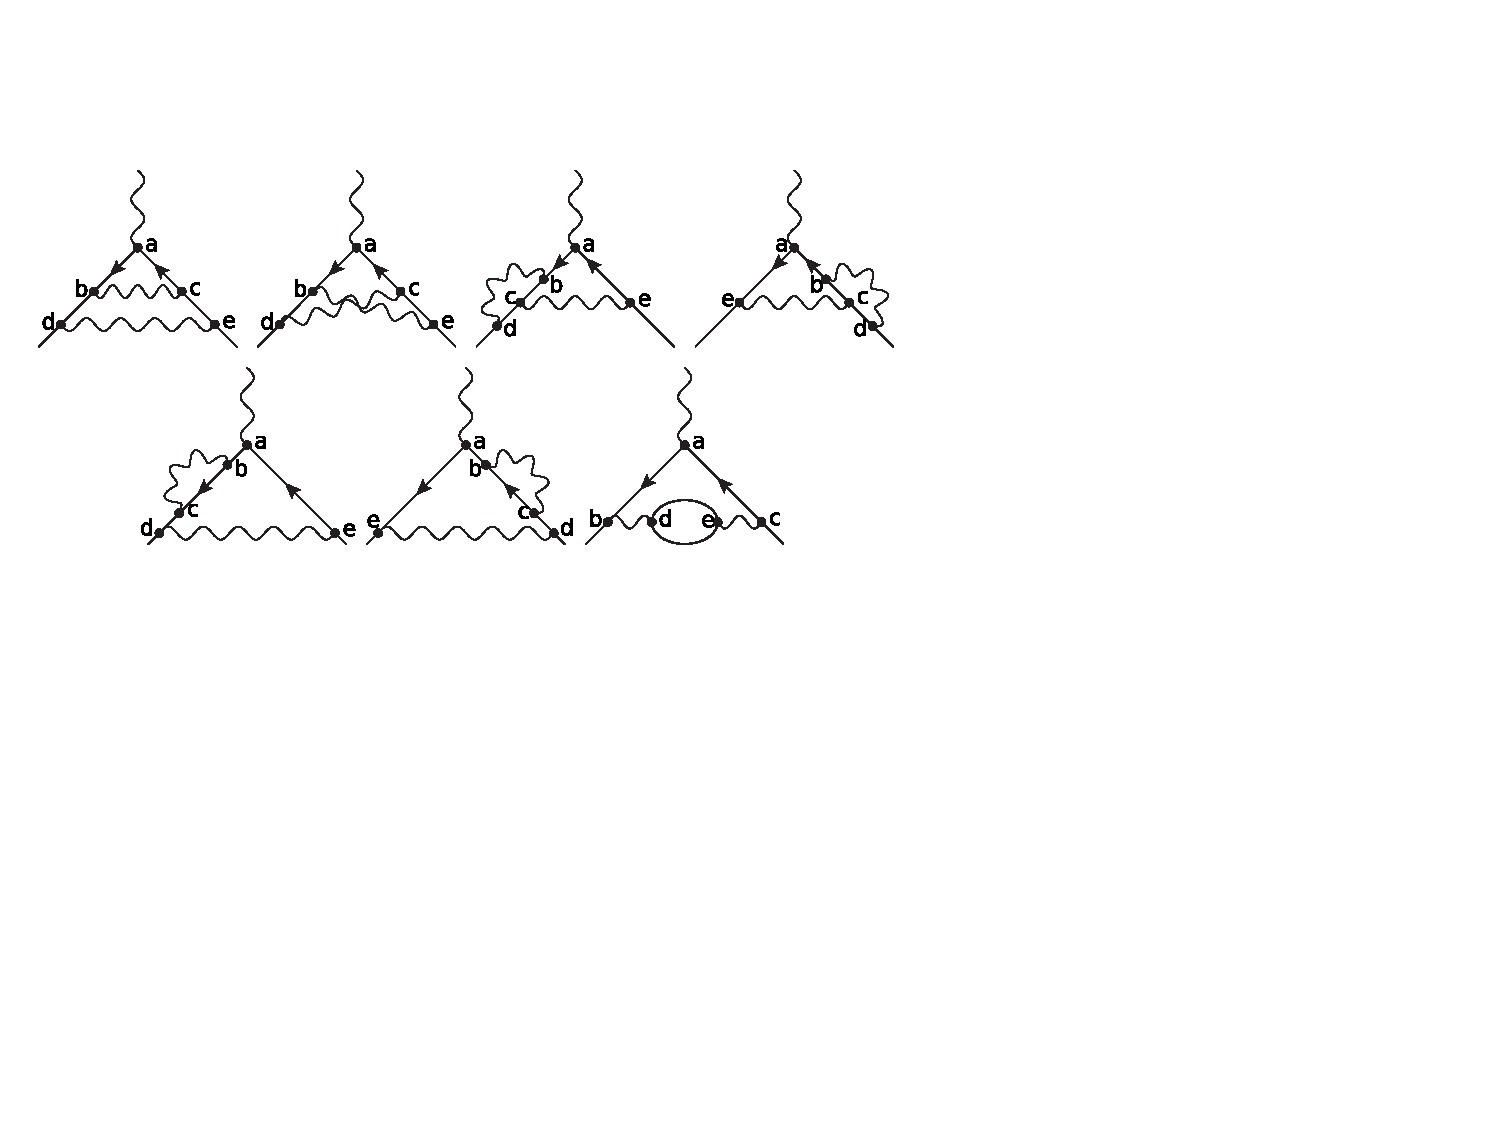
\includegraphics[width=0.50\textwidth]{Volkov18twoLoops}
\end{center}
\caption{\label{Volkov18twoLoops}
The two-loop vertex diagrams contributing to $A^{(4)}$ magnetic moment
anomaly.
From Volvkov\rf{Volkov18}.
}
 \end{figure}
%%%%%%%%%%%%%%%%%%%%%%%%%%%%%%%%%%%%%%%%



\section{Gauge sets}
\label{sect:finitness}

\begin{bartlett}{
Is there any method of computing the anomalous moment of the
electron which, on first approximation, gives a fair approximation to the
$\alpha$ term and a crude one to $\alpha^2$; and when improved, increases
the accuracy of the $\alpha^2$ term, yielding a rough estimate to
$\alpha^3$ and beyond?
        }
\bauthor{
Feynman's challenge, 12th Solvay Conference\rf{Feynman62}
    }
\end{bartlett}

\bigskip

%%%%%%%%%%%%%%%%%%%%%%%%%%%%%%%%%%%%%%%%
\begin{figure}
\begin{center}
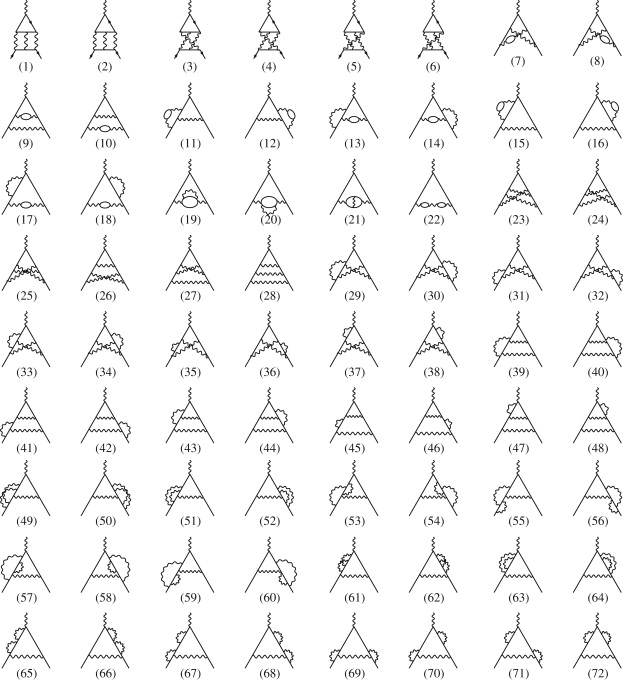
\includegraphics[width=1.00\textwidth]{JegNif09fig10}
\end{center}
\caption{\label{JegNif09fig10}
The three-loop vertex diagrams contributing to $A^{(6)}_1$
magnetic moment
(from Jegerlehner and Nyffeler\rf{JegNif09}).
Lautrup \etal\rf{LaPeRa72} were the first to note that
subsets
% $km'm$ =
$(3,0,0)$ = $\{23,24,25,26,27,28\}$;
$(2,1,0)$ = $\{29,31,33,35,37,39,41,43,45,47\}$ and its time-reversal
$(2,0,1)$ = $\{30,32,34,36,38,40,42,44,46,48\}$;
$(1,2,0)$ = $\{49,51,53,55,57,59,61,63,65,67\}$ and its time-reversal
$(1,0,2)$ = $\{50,52,54,56,58,60,62,64,66,68\}$;
and
$(1,1,1)$ = $\{69,70,71,72\}$
are the minimal gauge sets, see \reffig{Cvit77bFig2}.
}
 \end{figure}
%%%%%%%%%%%%%%%%%%%%%%%%%%%%%%%%%%%%%%%%

%%%%%%%%%%%%%%%%%%%%%%%%%%%%%%%%%%%%%%%%%%
\begin{table}
\begin{center}
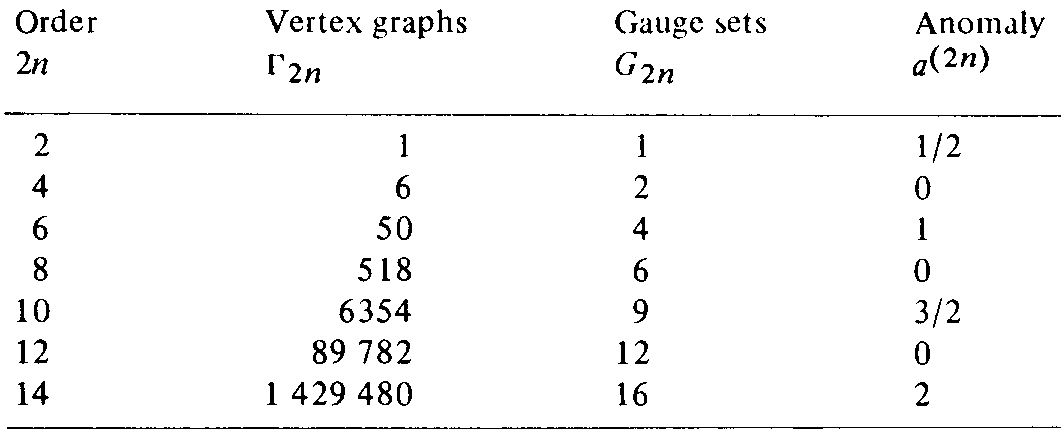
\includegraphics[width=0.80\textwidth]{Cvit77bTab1}
\end{center}
\caption{\label{Cvit77bTab1}
Comparison of the number of vertex diagrams without fermion loops, gauge
sets, and the gauge-set approximation \refeq{Cvit77b(1)} for the magnetic
moment in $2n$th order.
From \refref{Cvit77b}.
}
\end{table}
%%%%%%%%%%%%%%%%%%%%%%%%%%%%%%%%%%%%%%%%%%%%%%%%%%%%%%%%%%%

% finiteQEDins.tex
% PC created from lectures/talks/DFS_pris.tex       2017-05-25
% PC with edits March 2003
% PC with edits July 1997
%Acceptance speech - 1993 NKT Research Prize in Physics
%Dansk Fysisk Selskab \AA rsm\o de, Lalandia, R\o dby, 18 maj 1993
\noindent
In 1972 Toichiro Kinoshita and Predrag Cvitanovi\'c had completed
computing a large number of 3-loop anomalous magnetic moment Feynman
diagrams and regularization counterterms\rf{CviKin72},
\reffig{JegNif09fig10}.
The subsequent 4- and 5-loop numerical and analytic calculations were
nothing short of heroic\rf{KinLin90,LapRem96,Laporta17,AoHaKiNi15}. The
quantum field theory was used in the standard way\rf{BjoDre65}, by
expanding the magnetic moment into combinatorially many Feynman diagrams
(see the numbers of vertex graphs in \reftab{Cvit77bTab1}).
Each Feynman diagram corresponds to an integral in many dimensions, with
oscillatory integrand with thousands of terms, each integral separately
UV divergent, IR divergent, and unphysical, as its value depends on the
definition of counterterms and the choice of gauge.
The numerical values of these integrals typically range from  $\pm 10$
to $\pm 100$. For example, the largest contributions of
the 389 quenched self-energy diagrams listed in
Aoyama \etal\ 2018\rf{AoKiNi18} are of order $\pm 20$.

Adding up hundreds of such contributions, of wildly fluctuating values,
yields (for the no-fermion loops subset $V$, in the notation of
\refref{AoHaKiNi15})
\[
 \aql{6}\,=\, +  (0.92 \pm 0.02) \left(\frac{\alpha}{\pi}\right)^3.
\]
But why ``+'' and not ``-''? Why so small? Why does a sum of hundreds of
diagrams and counterterms yield a number of order of unity, and not 10 or
100 or any other number?

%%%%%%%%%%%%%%%%%%%%%%%%%%%%%%%%%%%%%%%%
\begin{figure}
\begin{center}
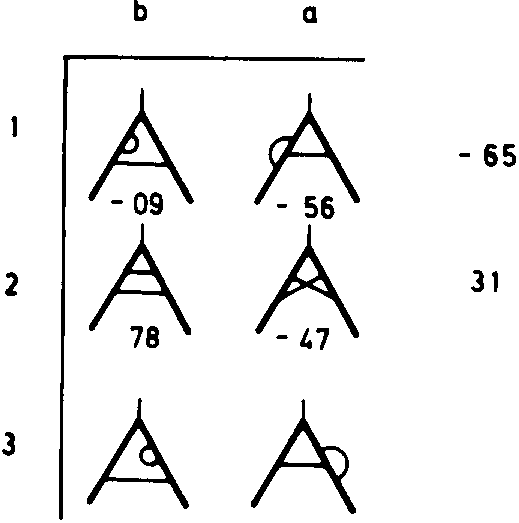
\includegraphics[width=0.50\textwidth]{Cvit77bFig1}
\end{center}
\caption{\label{Cvit77bFig1}
Rows: the fourth-order gauge sets
$km'm$: (1) = $(1,1,0)$,
(2) = $(2,0,0)$
and
(3) = $(1,0,1)$.
Columns: external field insertions into the two self-energy sets.
For diagrams related by time
reversal (here (1) and (3))
the value listed under the first diagram of the pair is
the total contribution of the pair. Contributions seem to be of order
$\pm\frac{1}{3}\left(\frac{\alpha}{\pi}\right)^2$, and suggest that
a set and its time-reversed partner should be counted separately.
From \refref{Cvit77b}.
}
 \end{figure}
%%%%%%%%%%%%%%%%%%%%%%%%%%%%%%%%%%%%%%%%

If gauge invariance of QED guarantees that all UV and on-mass shell IR
divergences cancel, could it be that it also enforces cancellations among
the finite parts of contributions of different Feynman graphs?

\subsection{QED vertex photons come in three ``colors''}
\label{sect:gaugeSetDeriv}

As first noted by Lautrup, Peterman and de Rafael\rf{LaPeRa72}, the
renormalized on-mass shell QED vertex diagrams separate into a sum of
minimal gauge-invariant subsets, each subset separately UV and IR finite.
The only published proof of this elementary fact seems to be
\refref{Cvit77b}. The very reasonably priced \refref{FieldThe} might be
worth a read, especially if one is interested in the non-abelian
theories as well\rf{MassShell,IRstruct,QCDmshell},
see \refsect{sect:QCDgaugeSets}.

A gauge change generates a $k^\mu$ term in a photon propagator,
and that affects a tree electron vertex in a very simple way,
\(
\slashed{k} = (\slashed{p}+\slashed{k}+m) - (\slashed{p}+m)
\,,
\)
or, diagrammatically\rf{BjoDre65,FieldThe} (graphs drawn by H.
Ki{\ss}ler\rf{KisKre16}),
\PC{2017-07-14
need to download, put axohelp.exe, the executable version of axohelp
for MS-Windows into the directory where I can run it from, presumably
Program~Files/MiKTeX 2.9/miktex/bin/x64
}
\begin{align}
  \begin{tabular}{ccccc}
$\!{\begin{aligned}\frac{1}{\slashed{p}+\slashed{k}-m}\slashed{k}\frac{1}{\slashed{p}-m}\end{aligned}}$ &
$=$ &    $\!{\begin{aligned}\frac{1}{\slashed{p}-m}\end{aligned}}$ &
$-$ &    $\!{\begin{aligned}\frac{1}{\slashed{p}+\slashed{k}-m},\end{aligned}}$
\\
$\treeA{.45}$ & $=$ & $\treeB{.45}$ & $-$ & $\treeC{.45}$.
  \end{tabular}
  \label{KisKre16eq:treeLevel1}
\end{align}

To simplify matters, in what follows we shall consider only the
no-fermion loop diagrams, or `quenched-', or `q-type' diagrams
(`quenched', as this corresponds to the $N_f$-independent part of the
vertex amplitude in
QED with $N_f$ flavors).
The minimal gauge-invariant subsets without electron loops (see
\reffig{JegNif09fig10} diagrams $\{23-72\}$; \reffig{Cvit77bFig1};
\ref{Cvit77bFig2}; \ref{Cvit77bFig3}; and \ref{Laporta17figuragauShort})
will be hereafter be referred to as \emph{gauge sets}.

A gauge set $km'm$ consists of all 1-particle irreducible vertex
diagrams without electron loops, with $k$ photons crossing the external
vertex (cross-photons) and $m [m']$ photons originating and terminating
on the incoming [outgoing] electron leg (leg-photons), where $m\geq m'$.
For asymmetric pairs of sets, with $m\neq m'$, the contribution to the
anomaly $a_{kmm'}$ is, in the convention of \refref{Cvit77b}, the sum of
the set and its mirror (time-reversed) image,
\beq
a[V]=\left.\frac{1}{2}(g-2)\right|_V
       =  \sum_{k=1}^\infty\sum_{m=0}^\infty\sum_{m'=0}^m
          a_{kmm'}\left(\frac{\alpha}{\pi}\right)^{k+m+m'}
\,.
\ee{quenchAnom}

\subsection{The unreasonable smallness of gauge sets}
\label{sect:gaugeSetsSmall}

When the diagrams computed in \refref{CviKin74c} are grouped into
gauge sets, \reffig{Cvit77bFig1} to \reffig{Laporta17figuragauShort},
a surprising thing happens; while the
finite part of each Feynman diagram is of order of 10 to 100, every
 gauge set known at the time added up to approximately
$$
		   \pm {1 \over 2} \left(\frac{\alpha}{\pi}\right)^n
\,,
$$
with the sign given by a simple empirical rule
\beq
a_{kmm'} = (-1)^{m+m'}\frac{1}{2}
\,.
\ee{Cvit77b(5)}
The sign rule is further corroborated by sets with photon
self-energy insertions (but with the absolute size scaled down to
$3-15\%$ of \refeq{Cvit77b(5)}).
In \reffig{Cvit77bFig3} this rule is compared with the actual numbers,
and the 1977 four-loop prediction is given\rf{Cvit77b}.
With that prediction, the ``zeroth'' order estimate of the electron
magnetic moment anomaly $a$ is given by the ``gauge-set
approximation,'' convergent and summable to all orders
\beq
a=\frac{1}{2}(g-2) =  \frac{1}{2} \frac{\alpha}{\pi}
                     \frac{1}
           {\left( 1 - \left(\frac{\alpha}{\pi}\right)^2
			\right)^2
		      } + \mbox{``corrections"}
\,.
\ee{Cvit77b(1)}
This is not how one usually thinks of perturbation theory. Most of our
colleagues believe that in 1952 Dyson\rf{Dyson52} had  shown that the
perturbation expansion is an asymptotic series (for a discussion, see
Dunne and Schubert\rf{DunSch06,HuTrSc17a}), in the sense that the $n$-th order
contribution should be exploding combinatorially
$$
{1 \over 2} (g-2) \approx
\cdots + n^n \left(\frac{\alpha}{\pi}\right)^n + \cdots
\,,
$$
and not growing slowly like my estimate
\[
{1 \over 2} (g-2) \approx
\cdots + \frac{n}{2}\left(\frac{\alpha}{\pi}\right)^{2n} + \cdots
\,.
\]
For me, the above is the most intriguing hint that something deeper than
what we know today underlies quantum field theory, and the most suggestive
lesson of our calculation.

%%%%%%%%%%%%%%%%%%%%%%%%%%%%%%%%%%%%%%%%%%%%%%%%%%%%%%%%
\begin{sidewaysfigure}[p]
\thisfloatpagestyle{empty} % Lucy Day Apr 18 2008
\center{
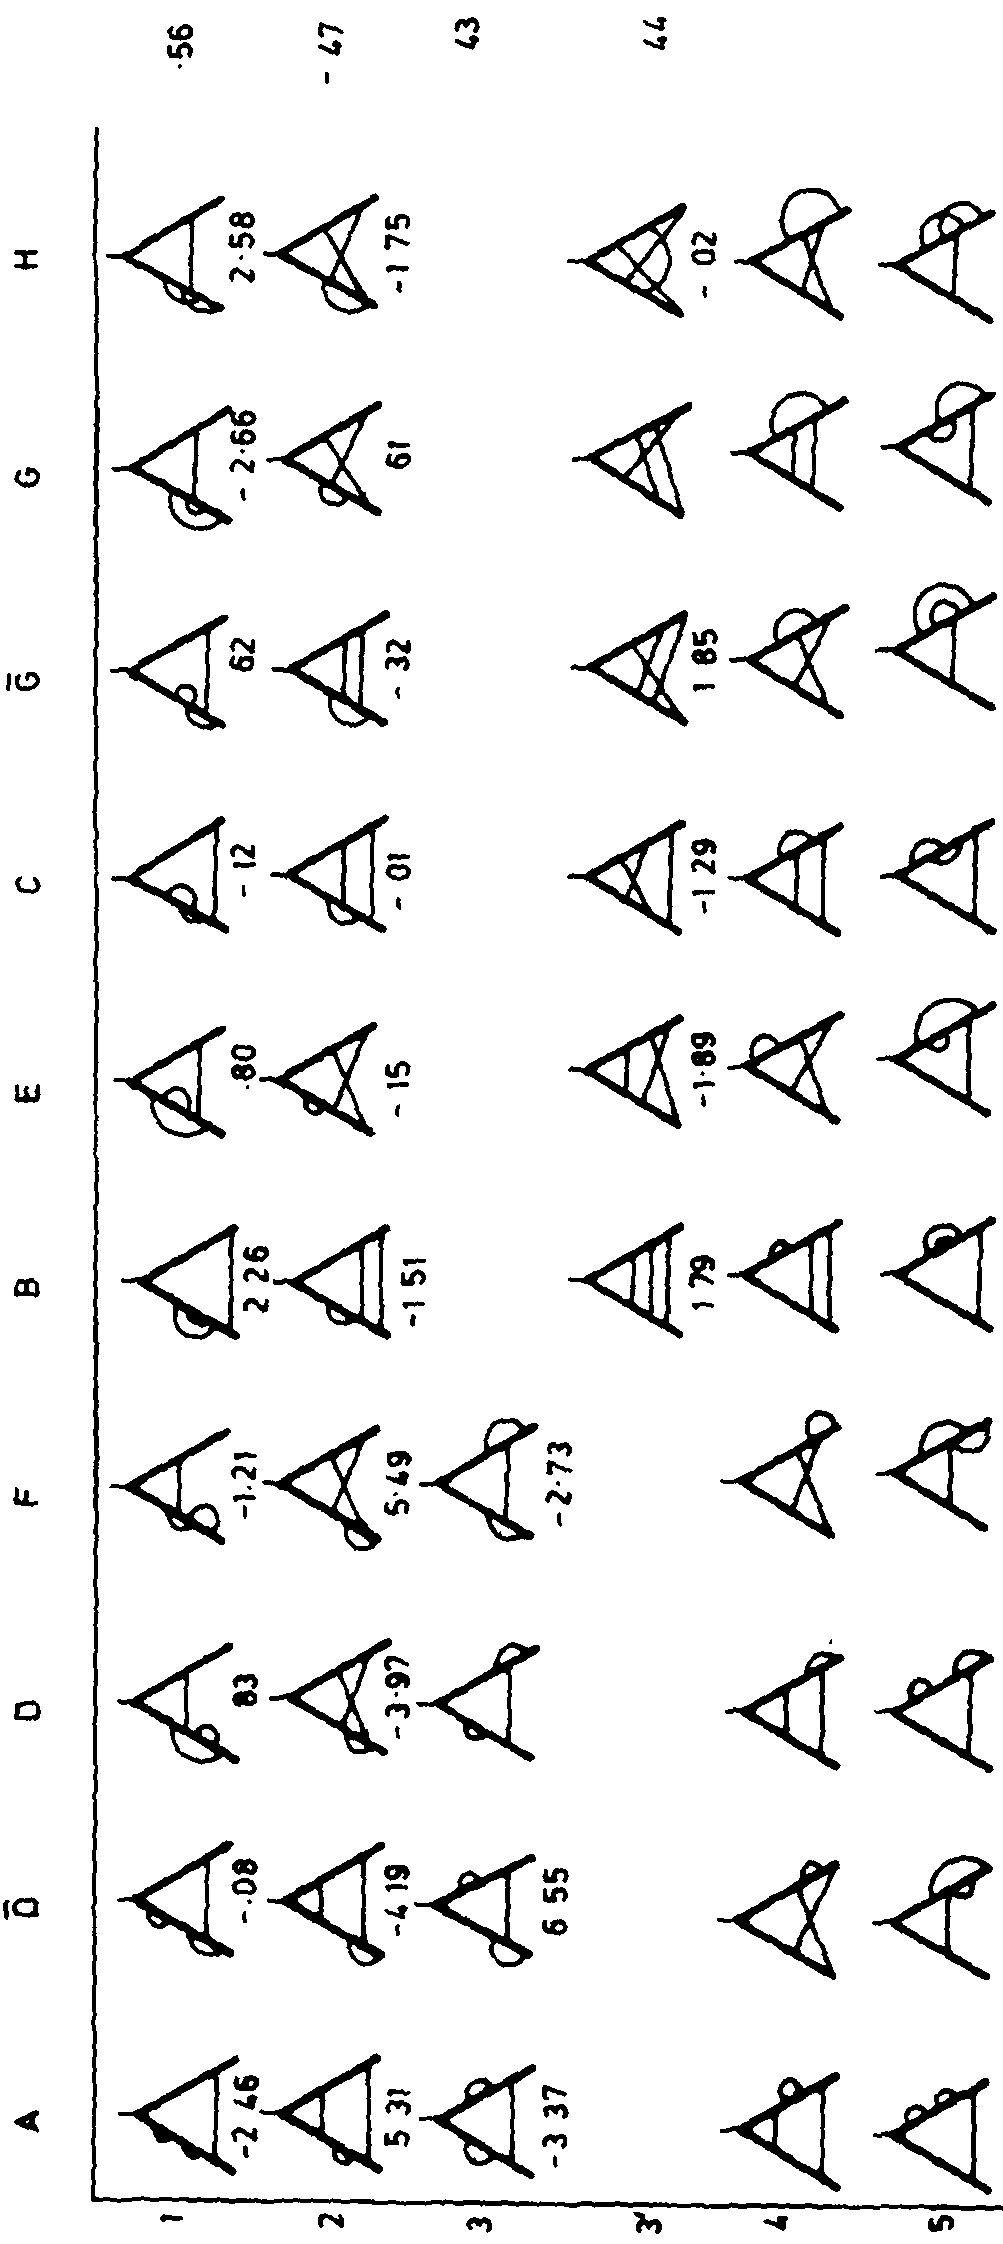
\includegraphics[width=0.44\textwidth,angle=-90]{Cvit77bFig2}
%\end{center}
        } %end \center{
\caption{\label{Cvit77bFig2}
Every vertex diagram belongs both to a `gauge set' and to a `self-energy set'.
This table illustrates the two kinds of sets.
The 3-loop gauge sets $km'm$ are arranged in the rows, and the
self-energy sets (or the `externally gauge-invariant' sets, vertex diagrams
obtained by inserting an extra vertex into a self-energy diagram) in the
columns, labeled as in Fig.~3 of \refref{CviKin74c}. The values are
finite parts in the $\ln\lambda$ IR cut-off approach, such as those
listed in \refref{LevWri73}. For different IR separation methods (such as
in \refref{CviKin74c}) and different gauges, individual diagrams have
different values. The gauge sets, however, are separately gauge invariant.
The self-energy sets (whose number grows combinatorially with the order
in perturbation theory) are not, only their sum is gauge invariant.
From \refref{Cvit77b}.
}
 \end{sidewaysfigure}
%%%%%%%%%%%%%%%%%%%%%%%%%%%%%%%%%%%%%%%%

%%%%%%%%%%%%%%%%%%%%%%%%%%%%%%%%%%%%%%%%
\begin{figure}
\begin{center}
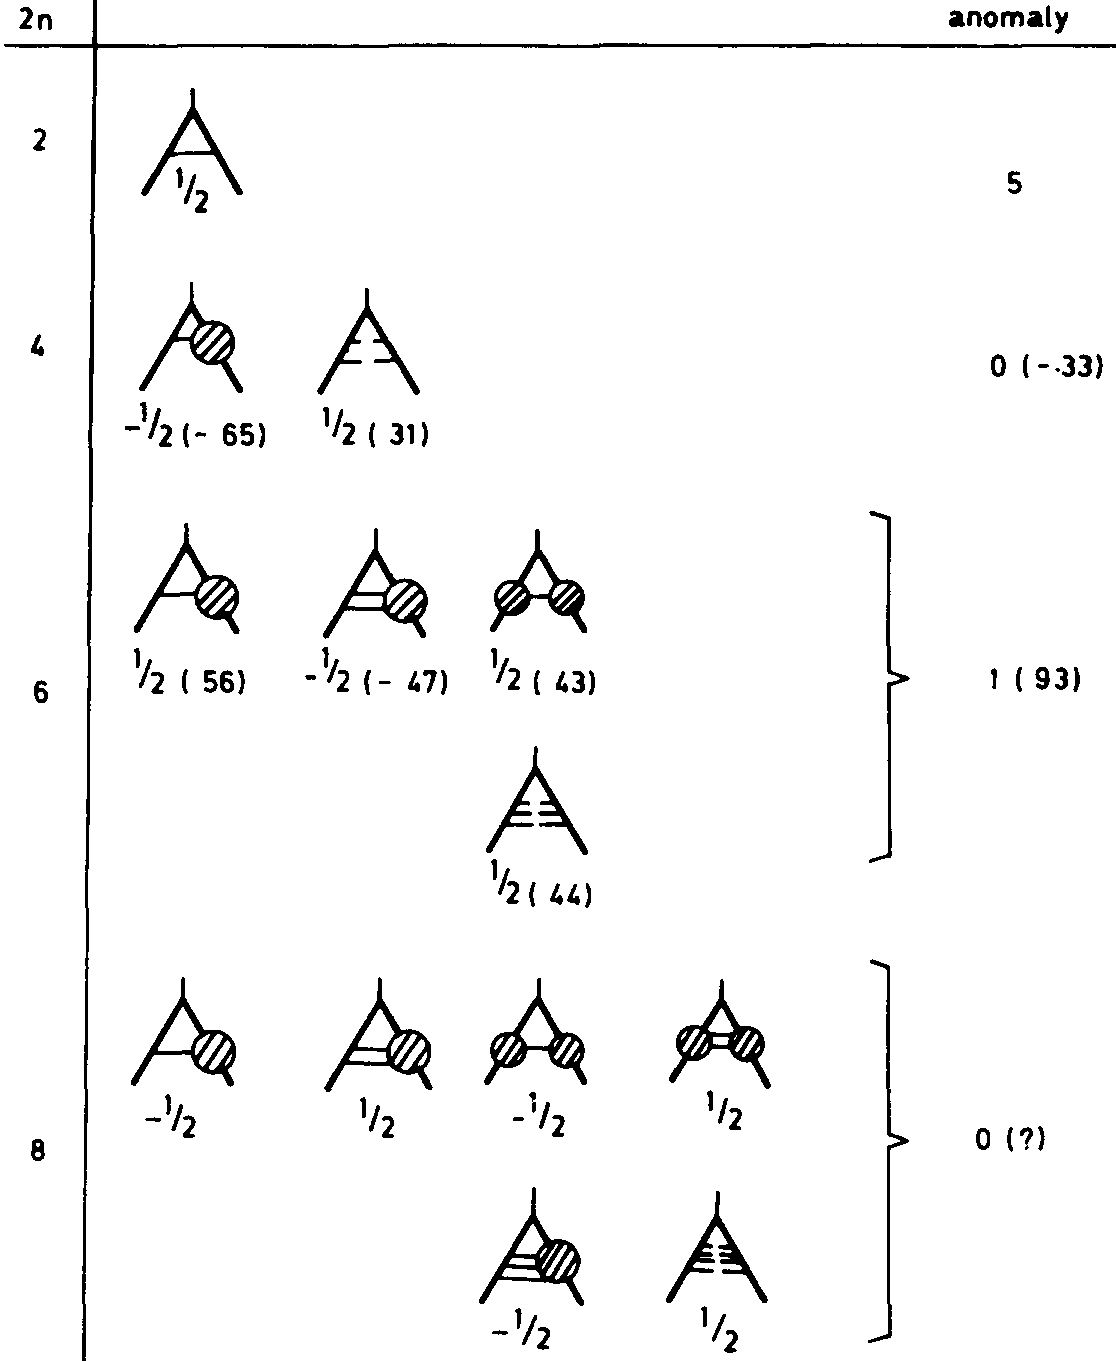
\includegraphics[width=0.90\textwidth]{Cvit77bFig3}
\end{center}
\caption{\label{Cvit77bFig3}
Comparison of the 1977 gauge-set approximation to the anomaly $a$
and the actual numerical
values of corresponding gauge sets, together with the  1977 eighth-order
prediction of \refref{Cvit77b}. For the updated listing, see
\reffig{tabGaugeSets}.
}
 \end{figure}
%%%%%%%%%%%%%%%%%%%%%%%%%%%%%%%%%%%%%%%%

%%%%%%%%%%%%%%%%%%%%%%%%%%%%%%%%%%%%%%%%%%
%%%%%%%%%%%%%%%%%%%%%%%%%%%%%%%%%%%%%%%%%%%%%%%%%%%%%
% tabGaugeSets.tex    2017-06-02
% compiled by  reducesymm/QFT/blog.tex
% needs \usepackage{booktabs}\usepackage{amsmath}
\begin{table}
\centering
{\small
\begin{tabular}{r@{~~~~}ccccc@{~~~~}l}
$2n$ & \multicolumn{5}{c}{$(k,m,m')$} & anomaly \\
    \toprule[1.5pt]\\[-1.0em]
% Entering  row 2
 & $\bf (1,0,0)$
 \\[-1ex]
\raisebox{1.5ex}{2}
 & $\frac{1}{2}$            &&&&& \raisebox{1.5ex}{$\frac{1}{2}$}
  \\[1ex]
 \cmidrule(lr){2-3}\\[-0.8em]
% Entering  row 4
 & $\bf (1,1,0)$  &  $\bf (2,0,0)$
 \\[-1ex]
\raisebox{1.5ex}{4}
 & -$\frac{1}{2}$ (-.65)&  $\frac{1}{2}$  (.31) &&&& \raisebox{1.5ex}{0 (-.33)}
  \\[1ex]
 \cmidrule(lr){2-4}\\[-0.8em]
% Entering  row 6
 & $\bf (1,2,0)$ & $\bf (2,1,0)$   & $\bf (3,0,0)$
 \\[0.1ex]
 & $\frac{1}{2}$ (.56) & -$\frac{1}{2}$ (-.47) &  $\frac{1}{2}$ (.44)
 \\%[-1ex]
\raisebox{1.5ex}{6}
 & $\bf (1,1,1)$ &&&&&          \raisebox{1.5ex}{1 (.93)}\\
 & $\frac{1}{2}$ (.43)
  \\[1ex]
 \cmidrule(lr){2-5}\\[-0.8em]
% Entering  row 8
 & $\bf (1,3,0)$     & $\bf (2,2,0)$  & $\bf (3,1,0)$  & $\bf (4,0,0)$
 \\[0.1ex]
 &  -$\frac{1}{2}${\color{red}$\cdot$4} (-1.97)
                     & $\frac{1}{2}${\color{red}$\cdot 0$ (-0.14)}
                                      & -$\frac{1}{2}${\color{red}$\cdot$2} (-1.04)
                                                        &  $\frac{1}{2}$ (.51)
 \\%[-1ex]
\raisebox{1.5ex}{8}
 & $\bf (1,2,1)$  & $\bf (2,1,1)$ &&&& \raisebox{1.5ex}{0 (-2.17)}\\
 & -$\frac{1}{2}$ (-.62)    &   $\frac{1}{2}${\color{red}$\cdot$2} (1.08)
  \\[1ex]
 \cmidrule(lr){2-6}
% Entering  row 10
 & $\bf (1,4,0)$ & $\bf (2,3,0)$  & $\bf (3,2,0)$
                                        & $\bf (4,1,0)$
                                            & $\bf (5,0,0)$
 \\[0.1ex]
 &    $\frac{1}{2}${\color{red}$\cdot$12} (6.2)
                 & -$\frac{1}{2}$ (-0.72)   & $\frac{1}{2}$  {\color{red} $\cdot 0$ (-0.40)}
                                        & -$\frac{1}{2}${\color{red}$\cdot$2} (-1.02)
                                             &  $\frac{1}{2}${\color{red}$\cdot$2} (1.09)
 \\%[-1ex]
\raisebox{1.5ex}{10}
 & $\bf (1,3,1)$  & $\bf (2,2,1)$ & $\bf (3,1,1)$ &&&
        \raisebox{1.5ex}{$\frac{3}{2} {\color{red} \cdot 4}\,(6.78)$}\\
 &  $\frac{1}{2}$ (0.90)    & -$\frac{1}{2}${\color{red}$\cdot$4} (-2.16)
                                  & $\frac{1}{2}${\color{red}$\cdot$5} (2.62)
  \\[1ex]
 & $\bf (1,2,2)$ \\
 & $\frac{1}{2}$ (0.30)
  \\[1ex]
\bottomrule
\end{tabular}
} %end {\small
\caption{\label{tabGaugeSets}
% Updated \reffig{Cvit77bFig3} comparison of
Comparison of the $\pm\frac{1}{2}$ gauge-set $(k,m,m')$ ansatz \refeq{Cvit77b(5)}
with the actual numerical value of corresponding gauge set, stated in $(\cdots)$
bracket.
Starting with 4-loops, the gauge-set ansatz \refeq{Cvit77b(5)} fails, but in
suggestive ways.
All gauge sets are surprisingly close to integer multiples of 1/2;
the ones differing from multiple 1 are marked in red.
The sign predictions are correct, except for the two anomalously small gauge sets
$(2,2,0)$, and its ``descendent'' $(3,2,0)$.
}
\end{table}
%%%%%%%%%%%%%%%%%%%%%%%%%%%%%%%%%%%%%%%%%%%%%%%%%%%%%

%%%%%%%%%%%%%%%%%%%%%%%%%%%%%%%%%%%%%%%%%%


%%%%%%%%%%%%%%%%%%%%%%%%%%%%%%%%%%%%%%%%%%
%% Laporta17figuragauShort.tex %%%%%
%% compiled by  reducesymm/QFT/blog.tex
%%%%%%%%%%%%%%%%%%%%%%%%%%%%%%%%%%%%%%%%
\begin{figure}[t]
\begin{center}
\begin{picture}(125,50)(70,350)
%\begin{picture}(125,30)(70,350)
\thicklines
%%%
{
\put(+000.0,+200.0){\makebox(0,0)[lb]{
% fotone obliquo (0.000000,200.000000) (0.000000,205.000000)
   \qbezier(+000.0,+200.0)(+001.2,+201.2)(+000.0,+202.5)
   \qbezier(+000.0,+202.5)(-001.2,+203.8)(+000.0,+205.0)
% elettrone curvo (0.000000,200.000000) (-20.000000,160.000000) 1000.000000
% cerchio r=44721.365140 c=(-40010.000000,20180.000000) ang=(-26.536403,-26.593699)
   \qbezier(+000.0,+200.0)(-010.0,+180.0)(-020.0,+160.0)
% elettrone curvo (0.000000,200.000000) (20.000000,160.000000) 1000.000000
% cerchio r=44721.365140 c=(-39990.000000,-19820.000000) ang=(26.593699,26.536403)
   \qbezier(+000.0,+200.0)(+010.0,+180.0)(+020.0,+160.0)
% fotone obliquo (-14.142136,171.715729) (14.142136,171.715729)
   \qbezier(-014.1,+171.7)(-013.3,+170.8)(-012.4,+171.7)
   \qbezier(-012.4,+171.7)(-011.5,+172.6)(-010.6,+171.7)
   \qbezier(-010.6,+171.7)(-009.7,+170.8)(-008.8,+171.7)
   \qbezier(-008.8,+171.7)(-008.0,+172.6)(-007.1,+171.7)
   \qbezier(-007.1,+171.7)(-006.2,+170.8)(-005.3,+171.7)
   \qbezier(-005.3,+171.7)(-004.4,+172.6)(-003.5,+171.7)
   \qbezier(-003.5,+171.7)(-002.7,+170.8)(-001.8,+171.7)
   \qbezier(-001.8,+171.7)(-000.9,+172.6)(+000.0,+171.7)
   \qbezier(+000.0,+171.7)(+000.9,+170.8)(+001.8,+171.7)
   \qbezier(+001.8,+171.7)(+002.7,+172.6)(+003.5,+171.7)
   \qbezier(+003.5,+171.7)(+004.4,+170.8)(+005.3,+171.7)
   \qbezier(+005.3,+171.7)(+006.2,+172.6)(+007.1,+171.7)
   \qbezier(+007.1,+171.7)(+008.0,+170.8)(+008.8,+171.7)
   \qbezier(+008.8,+171.7)(+009.7,+172.6)(+010.6,+171.7)
   \qbezier(+010.6,+171.7)(+011.5,+170.8)(+012.4,+171.7)
   \qbezier(+012.4,+171.7)(+013.3,+172.6)(+014.1,+171.7)
% fotone curvo (5.303301,189.393398) (10.000000,180.000000) 0.100000
% fotone semicircolare r=5.355061 c=(6.712311,184.227029) ang=(105.255119,-52.125016)
% n=8
   \qbezier(+005.3,+189.4)(+006.3,+188.7)(+007.1,+189.6)
   \qbezier(+007.1,+189.6)(+008.3,+190.3)(+008.9,+189.1)
   \qbezier(+008.9,+189.1)(+009.2,+187.9)(+010.4,+188.1)
   \qbezier(+010.4,+188.1)(+011.7,+187.9)(+011.5,+186.6)
   \qbezier(+011.5,+186.6)(+011.0,+185.5)(+012.0,+184.9)
   \qbezier(+012.0,+184.9)(+013.0,+183.9)(+011.9,+183.0)
   \qbezier(+011.9,+183.0)(+010.8,+182.5)(+011.2,+181.4)
   \qbezier(+011.2,+181.4)(+011.3,+180.0)(+010.0,+180.0)
% fotone curvo (12.247449,175.505103) (17.320508,165.358984) 0.100000
% fotone semicircolare r=5.784178 c=(13.769367,169.924737) ang=(105.255119,-52.125016)
% n=9
   \qbezier(+012.2,+175.5)(+013.2,+174.8)(+014.0,+175.7)
   \qbezier(+014.0,+175.7)(+015.0,+176.5)(+015.7,+175.4)
   \qbezier(+015.7,+175.4)(+016.1,+174.2)(+017.3,+174.5)
   \qbezier(+017.3,+174.5)(+018.6,+174.6)(+018.5,+173.3)
   \qbezier(+018.5,+173.3)(+018.2,+172.1)(+019.3,+171.7)
   \qbezier(+019.3,+171.7)(+020.3,+171.0)(+019.6,+170.0)
   \qbezier(+019.6,+170.0)(+018.6,+169.2)(+019.3,+168.2)
   \qbezier(+019.3,+168.2)(+019.8,+167.0)(+018.5,+166.6)
   \qbezier(+018.5,+166.6)(+017.3,+166.5)(+017.3,+165.4)
% fotone curvo (15.811388,168.377223) (18.708287,162.583426) -0.100000
% fotone semicircolare r=3.302973 c=(17.839217,165.770015) ang=(127.874984,285.255119)
% n=5
   \qbezier(+015.8,+168.4)(+014.5,+168.2)(+014.7,+166.9)
   \qbezier(+014.7,+166.9)(+015.4,+166.0)(+014.6,+165.1)
   \qbezier(+014.6,+165.1)(+014.1,+163.9)(+015.4,+163.5)
   \qbezier(+015.4,+163.5)(+016.5,+163.7)(+016.9,+162.6)
   \qbezier(+016.9,+162.6)(+017.8,+161.6)(+018.7,+162.6)
\put(+000.0,+152.0){\makebox(0,0){$(1)$}}
}}
\put(+025.0,+200.0){\makebox(0,0)[lb]{
% fotone obliquo (25.000000,200.000000) (25.000000,205.000000)
   \qbezier(+025.0,+200.0)(+026.2,+201.2)(+025.0,+202.5)
   \qbezier(+025.0,+202.5)(+023.8,+203.8)(+025.0,+205.0)
% elettrone curvo (25.000000,200.000000) (5.000000,160.000000) 1000.000000
% cerchio r=44721.365140 c=(-39985.000000,20180.000000) ang=(-26.536403,-26.593699)
   \qbezier(+025.0,+200.0)(+015.0,+180.0)(+005.0,+160.0)
% elettrone curvo (25.000000,200.000000) (45.000000,160.000000) 1000.000000
% cerchio r=44721.365140 c=(-39965.000000,-19820.000000) ang=(26.593699,26.536403)
   \qbezier(+025.0,+200.0)(+035.0,+180.0)(+045.0,+160.0)
% fotone obliquo (14.309550,178.619101) (35.690450,178.619101)
   \qbezier(+014.3,+178.6)(+015.2,+177.7)(+016.1,+178.6)
   \qbezier(+016.1,+178.6)(+017.0,+179.5)(+017.9,+178.6)
   \qbezier(+017.9,+178.6)(+018.8,+177.7)(+019.7,+178.6)
   \qbezier(+019.7,+178.6)(+020.5,+179.5)(+021.4,+178.6)
   \qbezier(+021.4,+178.6)(+022.3,+177.7)(+023.2,+178.6)
   \qbezier(+023.2,+178.6)(+024.1,+179.5)(+025.0,+178.6)
   \qbezier(+025.0,+178.6)(+025.9,+177.7)(+026.8,+178.6)
   \qbezier(+026.8,+178.6)(+027.7,+179.5)(+028.6,+178.6)
   \qbezier(+028.6,+178.6)(+029.5,+177.7)(+030.3,+178.6)
   \qbezier(+030.3,+178.6)(+031.2,+179.5)(+032.1,+178.6)
   \qbezier(+032.1,+178.6)(+033.0,+177.7)(+033.9,+178.6)
   \qbezier(+033.9,+178.6)(+034.8,+179.5)(+035.7,+178.6)
% fotone obliquo (8.096915,166.193830) (41.903085,166.193830)
   \qbezier(+008.1,+166.2)(+009.0,+165.3)(+009.9,+166.2)
   \qbezier(+009.9,+166.2)(+010.8,+167.1)(+011.7,+166.2)
   \qbezier(+011.7,+166.2)(+012.5,+165.3)(+013.4,+166.2)
   \qbezier(+013.4,+166.2)(+014.3,+167.1)(+015.2,+166.2)
   \qbezier(+015.2,+166.2)(+016.1,+165.3)(+017.0,+166.2)
   \qbezier(+017.0,+166.2)(+017.9,+167.1)(+018.8,+166.2)
   \qbezier(+018.8,+166.2)(+019.7,+165.3)(+020.6,+166.2)
   \qbezier(+020.6,+166.2)(+021.4,+167.1)(+022.3,+166.2)
   \qbezier(+022.3,+166.2)(+023.2,+165.3)(+024.1,+166.2)
   \qbezier(+024.1,+166.2)(+025.0,+167.1)(+025.9,+166.2)
   \qbezier(+025.9,+166.2)(+026.8,+165.3)(+027.7,+166.2)
   \qbezier(+027.7,+166.2)(+028.6,+167.1)(+029.4,+166.2)
   \qbezier(+029.4,+166.2)(+030.3,+165.3)(+031.2,+166.2)
   \qbezier(+031.2,+166.2)(+032.1,+167.1)(+033.0,+166.2)
   \qbezier(+033.0,+166.2)(+033.9,+165.3)(+034.8,+166.2)
   \qbezier(+034.8,+166.2)(+035.7,+167.1)(+036.6,+166.2)
   \qbezier(+036.6,+166.2)(+037.5,+165.3)(+038.3,+166.2)
   \qbezier(+038.3,+166.2)(+039.2,+167.1)(+040.1,+166.2)
   \qbezier(+040.1,+166.2)(+041.0,+165.3)(+041.9,+166.2)
% fotone curvo (32.559289,184.881421) (38.093073,173.813853) 0.100000
% fotone semicircolare r=6.309484 c=(34.219425,178.794259) ang=(105.255119,-52.125016)
% n=9
   \qbezier(+032.6,+184.9)(+033.6,+184.1)(+034.5,+185.1)
   \qbezier(+034.5,+185.1)(+035.6,+185.9)(+036.3,+184.7)
   \qbezier(+036.3,+184.7)(+036.8,+183.5)(+038.0,+183.8)
   \qbezier(+038.0,+183.8)(+039.4,+183.8)(+039.4,+182.4)
   \qbezier(+039.4,+182.4)(+039.0,+181.2)(+040.2,+180.7)
   \qbezier(+040.2,+180.7)(+041.4,+179.9)(+040.5,+178.8)
   \qbezier(+040.5,+178.8)(+039.5,+178.0)(+040.2,+176.9)
   \qbezier(+040.2,+176.9)(+040.7,+175.6)(+039.4,+175.2)
   \qbezier(+039.4,+175.2)(+038.1,+175.1)(+038.1,+173.8)
% fotone curvo (40.118579,169.762842) (43.516402,162.967196) 0.100000
% fotone semicircolare r=3.874114 c=(41.137926,166.025237) ang=(105.255119,-52.125016)
% n=6
   \qbezier(+040.1,+169.8)(+041.0,+169.0)(+041.9,+169.8)
   \qbezier(+041.9,+169.8)(+043.1,+170.3)(+043.5,+169.1)
   \qbezier(+043.5,+169.1)(+043.5,+168.0)(+044.6,+167.8)
   \qbezier(+044.6,+167.8)(+045.7,+167.1)(+045.0,+166.0)
   \qbezier(+045.0,+166.0)(+044.1,+165.4)(+044.6,+164.3)
   \qbezier(+044.6,+164.3)(+044.8,+163.0)(+043.5,+163.0)
\put(+025.0,+152.0){\makebox(0,0){$(2)$}}
}}
\put(+050.0,+200.0){\makebox(0,0)[lb]{
% fotone obliquo (50.000000,200.000000) (50.000000,205.000000)
   \qbezier(+050.0,+200.0)(+051.2,+201.2)(+050.0,+202.5)
   \qbezier(+050.0,+202.5)(+048.8,+203.8)(+050.0,+205.0)
% elettrone curvo (50.000000,200.000000) (30.000000,160.000000) 1000.000000
% cerchio r=44721.365140 c=(-39960.000000,20180.000000) ang=(-26.536403,-26.593699)
   \qbezier(+050.0,+200.0)(+040.0,+180.0)(+030.0,+160.0)
% elettrone curvo (50.000000,200.000000) (70.000000,160.000000) 1000.000000
% cerchio r=44721.365140 c=(-39940.000000,-19820.000000) ang=(26.593699,26.536403)
   \qbezier(+050.0,+200.0)(+060.0,+180.0)(+070.0,+160.0)
% fotone obliquo (33.670068,167.340137) (66.329932,167.340137)
   \qbezier(+033.7,+167.3)(+034.5,+166.5)(+035.4,+167.3)
   \qbezier(+035.4,+167.3)(+036.2,+168.2)(+037.1,+167.3)
   \qbezier(+037.1,+167.3)(+038.0,+166.5)(+038.8,+167.3)
   \qbezier(+038.8,+167.3)(+039.7,+168.2)(+040.5,+167.3)
   \qbezier(+040.5,+167.3)(+041.4,+166.5)(+042.3,+167.3)
   \qbezier(+042.3,+167.3)(+043.1,+168.2)(+044.0,+167.3)
   \qbezier(+044.0,+167.3)(+044.8,+166.5)(+045.7,+167.3)
   \qbezier(+045.7,+167.3)(+046.6,+168.2)(+047.4,+167.3)
   \qbezier(+047.4,+167.3)(+048.3,+166.5)(+049.1,+167.3)
   \qbezier(+049.1,+167.3)(+050.0,+168.2)(+050.9,+167.3)
   \qbezier(+050.9,+167.3)(+051.7,+166.5)(+052.6,+167.3)
   \qbezier(+052.6,+167.3)(+053.4,+168.2)(+054.3,+167.3)
   \qbezier(+054.3,+167.3)(+055.2,+166.5)(+056.0,+167.3)
   \qbezier(+056.0,+167.3)(+056.9,+168.2)(+057.7,+167.3)
   \qbezier(+057.7,+167.3)(+058.6,+166.5)(+059.5,+167.3)
   \qbezier(+059.5,+167.3)(+060.3,+168.2)(+061.2,+167.3)
   \qbezier(+061.2,+167.3)(+062.0,+166.5)(+062.9,+167.3)
   \qbezier(+062.9,+167.3)(+063.8,+168.2)(+064.6,+167.3)
   \qbezier(+064.6,+167.3)(+065.5,+166.5)(+066.3,+167.3)
% fotone curvo (35.857864,171.715729) (31.742581,163.485163) -0.100000
% fotone semicircolare r=4.692144 c=(34.623279,167.188917) ang=(74.744881,232.125016)
% n=7
   \qbezier(+035.9,+171.7)(+035.0,+172.8)(+034.0,+171.8)
   \qbezier(+034.0,+171.8)(+033.4,+170.8)(+032.3,+171.3)
   \qbezier(+032.3,+171.3)(+031.0,+171.4)(+030.9,+170.1)
   \qbezier(+030.9,+170.1)(+031.2,+168.9)(+030.1,+168.4)
   \qbezier(+030.1,+168.4)(+029.0,+167.6)(+030.0,+166.6)
   \qbezier(+030.0,+166.6)(+031.0,+166.0)(+030.5,+164.9)
   \qbezier(+030.5,+164.9)(+030.4,+163.5)(+031.7,+163.5)
% fotone curvo (64.142136,171.715729) (68.257419,163.485163) 0.100000
% fotone semicircolare r=4.692144 c=(65.376721,167.188917) ang=(105.255119,-52.125016)
% n=7
   \qbezier(+064.1,+171.7)(+065.1,+171.0)(+066.0,+171.8)
   \qbezier(+066.0,+171.8)(+067.1,+172.5)(+067.7,+171.3)
   \qbezier(+067.7,+171.3)(+067.9,+170.1)(+069.1,+170.1)
   \qbezier(+069.1,+170.1)(+070.4,+169.7)(+069.9,+168.4)
   \qbezier(+069.9,+168.4)(+069.2,+167.5)(+070.0,+166.6)
   \qbezier(+070.0,+166.6)(+070.7,+165.4)(+069.5,+164.9)
   \qbezier(+069.5,+164.9)(+068.2,+164.7)(+068.3,+163.5)
% fotone curvo (56.123724,187.752551) (61.547005,176.905989) 0.100000
% fotone semicircolare r=6.183492 c=(57.750709,181.786942) ang=(105.255119,-52.125016)
% n=9
   \qbezier(+056.1,+187.8)(+057.2,+187.0)(+058.0,+188.0)
   \qbezier(+058.0,+188.0)(+059.1,+188.8)(+059.8,+187.6)
   \qbezier(+059.8,+187.6)(+060.3,+186.4)(+061.5,+186.7)
   \qbezier(+061.5,+186.7)(+062.9,+186.7)(+062.8,+185.4)
   \qbezier(+062.8,+185.4)(+062.5,+184.1)(+063.6,+183.7)
   \qbezier(+063.6,+183.7)(+064.8,+182.9)(+063.9,+181.8)
   \qbezier(+063.9,+181.8)(+062.9,+181.0)(+063.7,+180.0)
   \qbezier(+063.7,+180.0)(+064.1,+178.7)(+062.8,+178.3)
   \qbezier(+062.8,+178.3)(+061.6,+178.2)(+061.5,+176.9)
\put(+050.0,+152.0){\makebox(0,0){$(3)$}}
}}
\put(+075.0,+200.0){\makebox(0,0)[lb]{
% fotone obliquo (75.000000,200.000000) (75.000000,205.000000)
   \qbezier(+075.0,+200.0)(+076.2,+201.2)(+075.0,+202.5)
   \qbezier(+075.0,+202.5)(+073.8,+203.8)(+075.0,+205.0)
% elettrone curvo (75.000000,200.000000) (55.000000,160.000000) 1000.000000
% cerchio r=44721.365140 c=(-39935.000000,20180.000000) ang=(-26.536403,-26.593699)
   \qbezier(+075.0,+200.0)(+065.0,+180.0)(+055.0,+160.0)
% elettrone curvo (75.000000,200.000000) (95.000000,160.000000) 1000.000000
% cerchio r=44721.365140 c=(-39915.000000,-19820.000000) ang=(26.593699,26.536403)
   \qbezier(+075.0,+200.0)(+085.0,+180.0)(+095.0,+160.0)
% fotone obliquo (66.835034,183.670068) (91.329932,167.340137)
   \qbezier(+066.8,+183.7)(+067.1,+182.5)(+068.3,+182.7)
   \qbezier(+068.3,+182.7)(+069.5,+182.9)(+069.7,+181.7)
   \qbezier(+069.7,+181.7)(+070.0,+180.5)(+071.2,+180.8)
   \qbezier(+071.2,+180.8)(+072.4,+181.0)(+072.6,+179.8)
   \qbezier(+072.6,+179.8)(+072.8,+178.6)(+074.0,+178.9)
   \qbezier(+074.0,+178.9)(+075.2,+179.1)(+075.5,+177.9)
   \qbezier(+075.5,+177.9)(+075.7,+176.7)(+076.9,+176.9)
   \qbezier(+076.9,+176.9)(+078.1,+177.2)(+078.4,+176.0)
   \qbezier(+078.4,+176.0)(+078.6,+174.8)(+079.8,+175.0)
   \qbezier(+079.8,+175.0)(+081.0,+175.3)(+081.2,+174.1)
   \qbezier(+081.2,+174.1)(+081.5,+172.9)(+082.7,+173.1)
   \qbezier(+082.7,+173.1)(+083.9,+173.3)(+084.1,+172.1)
   \qbezier(+084.1,+172.1)(+084.4,+170.9)(+085.6,+171.2)
   \qbezier(+085.6,+171.2)(+086.8,+171.4)(+087.0,+170.2)
   \qbezier(+087.0,+170.2)(+087.2,+169.0)(+088.4,+169.3)
   \qbezier(+088.4,+169.3)(+089.6,+169.5)(+089.9,+168.3)
   \qbezier(+089.9,+168.3)(+090.1,+167.1)(+091.3,+167.3)
% fotone obliquo (58.670068,167.340137) (83.164966,183.670068)
   \qbezier(+058.7,+167.3)(+059.9,+167.1)(+060.1,+168.3)
   \qbezier(+060.1,+168.3)(+060.4,+169.5)(+061.6,+169.3)
   \qbezier(+061.6,+169.3)(+062.8,+169.0)(+063.0,+170.2)
   \qbezier(+063.0,+170.2)(+063.2,+171.4)(+064.4,+171.2)
   \qbezier(+064.4,+171.2)(+065.6,+170.9)(+065.9,+172.1)
   \qbezier(+065.9,+172.1)(+066.1,+173.3)(+067.3,+173.1)
   \qbezier(+067.3,+173.1)(+068.5,+172.9)(+068.8,+174.1)
   \qbezier(+068.8,+174.1)(+069.0,+175.3)(+070.2,+175.0)
   \qbezier(+070.2,+175.0)(+071.4,+174.8)(+071.6,+176.0)
   \qbezier(+071.6,+176.0)(+071.9,+177.2)(+073.1,+176.9)
   \qbezier(+073.1,+176.9)(+074.3,+176.7)(+074.5,+177.9)
   \qbezier(+074.5,+177.9)(+074.8,+179.1)(+076.0,+178.9)
   \qbezier(+076.0,+178.9)(+077.2,+178.6)(+077.4,+179.8)
   \qbezier(+077.4,+179.8)(+077.6,+181.0)(+078.8,+180.8)
   \qbezier(+078.8,+180.8)(+080.0,+180.5)(+080.3,+181.7)
   \qbezier(+080.3,+181.7)(+080.5,+182.9)(+081.7,+182.7)
   \qbezier(+081.7,+182.7)(+082.9,+182.5)(+083.2,+183.7)
% fotone curvo (60.857864,171.715729) (56.742581,163.485163) -0.100000
% fotone semicircolare r=4.692144 c=(59.623279,167.188917) ang=(74.744881,232.125016)
% n=7
   \qbezier(+060.9,+171.7)(+060.0,+172.8)(+059.0,+171.8)
   \qbezier(+059.0,+171.8)(+058.4,+170.8)(+057.3,+171.3)
   \qbezier(+057.3,+171.3)(+056.0,+171.4)(+055.9,+170.1)
   \qbezier(+055.9,+170.1)(+056.2,+168.9)(+055.1,+168.4)
   \qbezier(+055.1,+168.4)(+054.0,+167.6)(+055.0,+166.6)
   \qbezier(+055.0,+166.6)(+056.0,+166.0)(+055.5,+164.9)
   \qbezier(+055.5,+164.9)(+055.4,+163.5)(+056.7,+163.5)
% fotone curvo (85.526385,178.947231) (89.142136,171.715729) 0.100000
% fotone semicircolare r=4.122590 c=(86.611110,174.969905) ang=(105.255119,-52.125016)
% n=6
   \qbezier(+085.5,+178.9)(+086.5,+178.2)(+087.4,+179.0)
   \qbezier(+087.4,+179.0)(+088.7,+179.6)(+089.1,+178.3)
   \qbezier(+089.1,+178.3)(+089.1,+177.0)(+090.3,+176.8)
   \qbezier(+090.3,+176.8)(+091.5,+176.1)(+090.7,+175.0)
   \qbezier(+090.7,+175.0)(+089.7,+174.3)(+090.3,+173.2)
   \qbezier(+090.3,+173.2)(+090.5,+171.8)(+089.1,+171.7)
\put(+075.0,+152.0){\makebox(0,0){$(4)$}}
}}
\put(+100.0,+200.0){\makebox(0,0)[lb]{
% fotone obliquo (100.000000,200.000000) (100.000000,205.000000)
   \qbezier(+100.0,+200.0)(+101.2,+201.2)(+100.0,+202.5)
   \qbezier(+100.0,+202.5)(+098.8,+203.8)(+100.0,+205.0)
% elettrone curvo (100.000000,200.000000) (80.000000,160.000000) 1000.000000
% cerchio r=44721.365140 c=(-39910.000000,20180.000000) ang=(-26.536403,-26.593699)
   \qbezier(+100.0,+200.0)(+090.0,+180.0)(+080.0,+160.0)
% elettrone curvo (100.000000,200.000000) (120.000000,160.000000) 1000.000000
% cerchio r=44721.365140 c=(-39890.000000,-19820.000000) ang=(26.593699,26.536403)
   \qbezier(+100.0,+200.0)(+110.0,+180.0)(+120.0,+160.0)
% fotone obliquo (91.835034,183.670068) (114.142136,171.715729)
   \qbezier(+091.8,+183.7)(+092.2,+182.4)(+093.4,+182.8)
   \qbezier(+093.4,+182.8)(+094.7,+183.2)(+095.0,+182.0)
   \qbezier(+095.0,+182.0)(+095.4,+180.7)(+096.6,+181.1)
   \qbezier(+096.6,+181.1)(+097.8,+181.5)(+098.2,+180.3)
   \qbezier(+098.2,+180.3)(+098.6,+179.0)(+099.8,+179.4)
   \qbezier(+099.8,+179.4)(+101.0,+179.8)(+101.4,+178.5)
   \qbezier(+101.4,+178.5)(+101.8,+177.3)(+103.0,+177.7)
   \qbezier(+103.0,+177.7)(+104.2,+178.1)(+104.6,+176.8)
   \qbezier(+104.6,+176.8)(+105.0,+175.6)(+106.2,+176.0)
   \qbezier(+106.2,+176.0)(+107.4,+176.4)(+107.8,+175.1)
   \qbezier(+107.8,+175.1)(+108.1,+173.9)(+109.4,+174.3)
   \qbezier(+109.4,+174.3)(+110.6,+174.6)(+111.0,+173.4)
   \qbezier(+111.0,+173.4)(+111.3,+172.2)(+112.5,+172.6)
   \qbezier(+112.5,+172.6)(+113.8,+172.9)(+114.1,+171.7)
% fotone obliquo (85.857864,171.715729) (108.164966,183.670068)
   \qbezier(+085.9,+171.7)(+087.1,+171.3)(+087.5,+172.6)
   \qbezier(+087.5,+172.6)(+087.8,+173.8)(+089.0,+173.4)
   \qbezier(+089.0,+173.4)(+090.3,+173.1)(+090.6,+174.3)
   \qbezier(+090.6,+174.3)(+091.0,+175.5)(+092.2,+175.1)
   \qbezier(+092.2,+175.1)(+093.5,+174.8)(+093.8,+176.0)
   \qbezier(+093.8,+176.0)(+094.2,+177.2)(+095.4,+176.8)
   \qbezier(+095.4,+176.8)(+096.6,+176.5)(+097.0,+177.7)
   \qbezier(+097.0,+177.7)(+097.4,+178.9)(+098.6,+178.5)
   \qbezier(+098.6,+178.5)(+099.8,+178.2)(+100.2,+179.4)
   \qbezier(+100.2,+179.4)(+100.6,+180.6)(+101.8,+180.3)
   \qbezier(+101.8,+180.3)(+103.0,+179.9)(+103.4,+181.1)
   \qbezier(+103.4,+181.1)(+103.8,+182.3)(+105.0,+182.0)
   \qbezier(+105.0,+182.0)(+106.2,+181.6)(+106.6,+182.8)
   \qbezier(+106.6,+182.8)(+106.9,+184.0)(+108.2,+183.7)
% fotone obliquo (81.742581,163.485163) (118.257419,163.485163)
   \qbezier(+081.7,+163.5)(+082.6,+162.6)(+083.5,+163.5)
   \qbezier(+083.5,+163.5)(+084.4,+164.4)(+085.2,+163.5)
   \qbezier(+085.2,+163.5)(+086.1,+162.6)(+087.0,+163.5)
   \qbezier(+087.0,+163.5)(+087.8,+164.4)(+088.7,+163.5)
   \qbezier(+088.7,+163.5)(+089.6,+162.6)(+090.4,+163.5)
   \qbezier(+090.4,+163.5)(+091.3,+164.4)(+092.2,+163.5)
   \qbezier(+092.2,+163.5)(+093.0,+162.6)(+093.9,+163.5)
   \qbezier(+093.9,+163.5)(+094.8,+164.4)(+095.7,+163.5)
   \qbezier(+095.7,+163.5)(+096.5,+162.6)(+097.4,+163.5)
   \qbezier(+097.4,+163.5)(+098.3,+164.4)(+099.1,+163.5)
   \qbezier(+099.1,+163.5)(+100.0,+162.6)(+100.9,+163.5)
   \qbezier(+100.9,+163.5)(+101.7,+164.4)(+102.6,+163.5)
   \qbezier(+102.6,+163.5)(+103.5,+162.6)(+104.3,+163.5)
   \qbezier(+104.3,+163.5)(+105.2,+164.4)(+106.1,+163.5)
   \qbezier(+106.1,+163.5)(+107.0,+162.6)(+107.8,+163.5)
   \qbezier(+107.8,+163.5)(+108.7,+164.4)(+109.6,+163.5)
   \qbezier(+109.6,+163.5)(+110.4,+162.6)(+111.3,+163.5)
   \qbezier(+111.3,+163.5)(+112.2,+164.4)(+113.0,+163.5)
   \qbezier(+113.0,+163.5)(+113.9,+162.6)(+114.8,+163.5)
   \qbezier(+114.8,+163.5)(+115.6,+164.4)(+116.5,+163.5)
   \qbezier(+116.5,+163.5)(+117.4,+162.6)(+118.3,+163.5)
% fotone curvo (111.547005,176.905989) (116.329932,167.340137) 0.100000
% fotone semicircolare r=5.453375 c=(112.981883,171.644770) ang=(105.255119,-52.125016)
% n=8
   \qbezier(+111.5,+176.9)(+112.6,+176.2)(+113.4,+177.1)
   \qbezier(+113.4,+177.1)(+114.6,+177.8)(+115.2,+176.6)
   \qbezier(+115.2,+176.6)(+115.5,+175.4)(+116.8,+175.6)
   \qbezier(+116.8,+175.6)(+118.1,+175.4)(+117.9,+174.1)
   \qbezier(+117.9,+174.1)(+117.3,+173.0)(+118.4,+172.3)
   \qbezier(+118.4,+172.3)(+119.3,+171.3)(+118.3,+170.4)
   \qbezier(+118.3,+170.4)(+117.2,+169.9)(+117.6,+168.7)
   \qbezier(+117.6,+168.7)(+117.7,+167.4)(+116.3,+167.3)
\put(+100.0,+152.0){\makebox(0,0){$(5)$}}
}}
\put(+250.0,+235.0){\makebox(0,0)[lb]{
% fotone obliquo (0.000000,165.000000) (0.000000,170.000000)
   \qbezier(+000.0,+165.0)(+001.2,+166.2)(+000.0,+167.5)
   \qbezier(+000.0,+167.5)(-001.2,+168.8)(+000.0,+170.0)
% elettrone curvo (0.000000,165.000000) (-20.000000,125.000000) 1000.000000
% cerchio r=44721.365140 c=(-40010.000000,20145.000000) ang=(-26.536403,-26.593699)
   \qbezier(+000.0,+165.0)(-010.0,+145.0)(-020.0,+125.0)
% elettrone curvo (0.000000,165.000000) (20.000000,125.000000) 1000.000000
% cerchio r=44721.365140 c=(-39990.000000,-19855.000000) ang=(26.593699,26.536403)
   \qbezier(+000.0,+165.0)(+010.0,+145.0)(+020.0,+125.0)
% fotone obliquo (-8.944272,147.111456) (12.649111,139.701779)
   \qbezier(-008.9,+147.1)(-008.4,+146.0)(-007.3,+146.5)
   \qbezier(-007.3,+146.5)(-006.2,+147.1)(-005.6,+146.0)
   \qbezier(-005.6,+146.0)(-005.1,+144.9)(-004.0,+145.4)
   \qbezier(-004.0,+145.4)(-002.8,+145.9)(-002.3,+144.8)
   \qbezier(-002.3,+144.8)(-001.8,+143.7)(-000.6,+144.3)
   \qbezier(-000.6,+144.3)(+000.5,+144.8)(+001.0,+143.7)
   \qbezier(+001.0,+143.7)(+001.6,+142.6)(+002.7,+143.1)
   \qbezier(+002.7,+143.1)(+003.8,+143.7)(+004.3,+142.6)
   \qbezier(+004.3,+142.6)(+004.9,+141.4)(+006.0,+142.0)
   \qbezier(+006.0,+142.0)(+007.1,+142.5)(+007.7,+141.4)
   \qbezier(+007.7,+141.4)(+008.2,+140.3)(+009.3,+140.8)
   \qbezier(+009.3,+140.8)(+010.4,+141.4)(+011.0,+140.3)
   \qbezier(+011.0,+140.3)(+011.5,+139.2)(+012.6,+139.7)
% fotone obliquo (-12.649111,139.701779) (15.491933,134.016133)
   \qbezier(-012.6,+139.7)(-011.9,+138.6)(-010.9,+139.3)
   \qbezier(-010.9,+139.3)(-009.8,+140.0)(-009.1,+139.0)
   \qbezier(-009.1,+139.0)(-008.4,+137.9)(-007.4,+138.6)
   \qbezier(-007.4,+138.6)(-006.3,+139.3)(-005.6,+138.3)
   \qbezier(-005.6,+138.3)(-004.9,+137.2)(-003.9,+137.9)
   \qbezier(-003.9,+137.9)(-002.8,+138.6)(-002.1,+137.6)
   \qbezier(-002.1,+137.6)(-001.4,+136.5)(-000.3,+137.2)
   \qbezier(-000.3,+137.2)(+000.7,+137.9)(+001.4,+136.9)
   \qbezier(+001.4,+136.9)(+002.1,+135.8)(+003.2,+136.5)
   \qbezier(+003.2,+136.5)(+004.2,+137.2)(+004.9,+136.1)
   \qbezier(+004.9,+136.1)(+005.6,+135.1)(+006.7,+135.8)
   \qbezier(+006.7,+135.8)(+007.8,+136.5)(+008.5,+135.4)
   \qbezier(+008.5,+135.4)(+009.2,+134.4)(+010.2,+135.1)
   \qbezier(+010.2,+135.1)(+011.3,+135.8)(+012.0,+134.7)
   \qbezier(+012.0,+134.7)(+012.7,+133.7)(+013.7,+134.4)
   \qbezier(+013.7,+134.4)(+014.8,+135.1)(+015.5,+134.0)
% fotone obliquo (-15.491933,134.016133) (17.888544,129.222912)
   \qbezier(-015.5,+134.0)(-014.7,+133.0)(-013.7,+133.8)
   \qbezier(-013.7,+133.8)(-012.7,+134.5)(-012.0,+133.5)
   \qbezier(-012.0,+133.5)(-011.2,+132.5)(-010.2,+133.3)
   \qbezier(-010.2,+133.3)(-009.2,+134.0)(-008.5,+133.0)
   \qbezier(-008.5,+133.0)(-007.7,+132.0)(-006.7,+132.8)
   \qbezier(-006.7,+132.8)(-005.7,+133.5)(-005.0,+132.5)
   \qbezier(-005.0,+132.5)(-004.2,+131.5)(-003.2,+132.3)
   \qbezier(-003.2,+132.3)(-002.2,+133.0)(-001.4,+132.0)
   \qbezier(-001.4,+132.0)(-000.7,+131.0)(+000.3,+131.7)
   \qbezier(+000.3,+131.7)(+001.3,+132.5)(+002.1,+131.5)
   \qbezier(+002.1,+131.5)(+002.8,+130.5)(+003.8,+131.2)
   \qbezier(+003.8,+131.2)(+004.8,+132.0)(+005.6,+131.0)
   \qbezier(+005.6,+131.0)(+006.3,+130.0)(+007.3,+130.7)
   \qbezier(+007.3,+130.7)(+008.4,+131.5)(+009.1,+130.5)
   \qbezier(+009.1,+130.5)(+009.9,+129.5)(+010.9,+130.2)
   \qbezier(+010.9,+130.2)(+011.9,+131.0)(+012.6,+130.0)
   \qbezier(+012.6,+130.0)(+013.4,+129.0)(+014.4,+129.7)
   \qbezier(+014.4,+129.7)(+015.4,+130.5)(+016.1,+129.5)
   \qbezier(+016.1,+129.5)(+016.9,+128.5)(+017.9,+129.2)
% fotone obliquo (-17.888544,129.222912) (8.944272,147.111456)
   \qbezier(-017.9,+129.2)(-016.6,+129.0)(-016.4,+130.2)
   \qbezier(-016.4,+130.2)(-016.1,+131.5)(-014.9,+131.2)
   \qbezier(-014.9,+131.2)(-013.7,+131.0)(-013.4,+132.2)
   \qbezier(-013.4,+132.2)(-013.2,+133.4)(-011.9,+133.2)
   \qbezier(-011.9,+133.2)(-010.7,+132.9)(-010.4,+134.2)
   \qbezier(-010.4,+134.2)(-010.2,+135.4)(-008.9,+135.2)
   \qbezier(-008.9,+135.2)(-007.7,+134.9)(-007.5,+136.2)
   \qbezier(-007.5,+136.2)(-007.2,+137.4)(-006.0,+137.2)
   \qbezier(-006.0,+137.2)(-004.7,+136.9)(-004.5,+138.2)
   \qbezier(-004.5,+138.2)(-004.2,+139.4)(-003.0,+139.2)
   \qbezier(-003.0,+139.2)(-001.7,+138.9)(-001.5,+140.2)
   \qbezier(-001.5,+140.2)(-001.2,+141.4)(-000.0,+141.1)
   \qbezier(+000.0,+141.1)(+001.2,+140.9)(+001.5,+142.1)
   \qbezier(+001.5,+142.1)(+001.7,+143.4)(+003.0,+143.1)
   \qbezier(+003.0,+143.1)(+004.2,+142.9)(+004.5,+144.1)
   \qbezier(+004.5,+144.1)(+004.7,+145.4)(+006.0,+145.1)
   \qbezier(+006.0,+145.1)(+007.2,+144.9)(+007.5,+146.1)
   \qbezier(+007.5,+146.1)(+007.7,+147.4)(+008.9,+147.1)
\put(+000.0,+117.0){\makebox(0,0){$(6)$}}
}}
}
%%%
 \end{picture}
  \\[3ex]
\begin{tabular}{ccrrr}
gauge set &$(k,m,m')$& value~~ & prediction \\
\hline
   (1)  & (1,3,0) & - 1.9710    & - 1/2  \\%01
   (2)  & (2,2,0) &  - 0.1424   & \phantom{+} 1/2 &~(!)\\%02
   (3)  & (1,2,1) &  - 0.6219   & - 1/2  \\%03
   (4)  & (2,1,1) &  \phantom{+} 1.0867  & \phantom{+} 1/2  \\%04
   (5)  & (3,1,0) &  - 1.0405   & - 1/2  \\%05
   (6)  & (4,0,0) &  \phantom{+} 0.5125  & \phantom{+} 1/2  \\%06
\hline
%  1+2+{\ldots}+6 & - 2.176866027739540077443259355895893938670  \\
% -2*1.9710-2*0.14249-2*0.6219+1.0867-2*1.0405+0.5125 =
% -1.9710-0.14249-0.6219+1.0867-1.0405+0.5125 =  -2.17669
\end{tabular}
 \end{center}
%%/ \phantom{ }\vspace{0truecm}\phantom{ }
\caption{\label{Laporta17figuragauShort}
(top)
Examples of 4-loop vertex diagrams belonging to Laporta\rf{Laporta17} gauge sets
(1) to (6).
%(1) = $(1,3,0)$,
%(2) = $(2,2,0)$,
%(3) = $(1,2,1)$,
%(4) = $(2,1,1)$,
%(5) = $(3,1,0)$,
%(6) = $(4,0,0)$.
The remaining diagrams in the set can be obtained by permuting separately
the vertices on the left and right side of the electron line, and
considering also the mirror images of the diagrams. For all 25
gauge-invariant sets, see \reffig{Laporta17figuragau}.
The table:
Gauge-set contributions $a^{(8)}_{kmm'}$, see \refeq{quenchAnom}, as
reported by Laporta\rf{Laporta17}
(for the full 25 gauge-invariant sets, see \reftab{Laporta17:tableset}).
The last column: 1977 Cvitanovi\'c predictions\rf{Cvit77b}.
Signs are right, except for the set (2) = $(2,2,0)$, which is anomalously
small, and the remaining sets are surprisingly close to multiples of 1/2.
There might be factors of 2 having to do with symmetries, missing from
the guesses of \refref{Cvit77b}, but I cannot see how that would work.
Only (4) = $(2,1,1)$ and  (6) = $(4,0,0)$ are symmetric,
but (1) = $(1,3,0)$, (4) and (5) = $(3,1,0)$ seem to
have an extra factor of 2 or 4.
}
 \end{figure}
%%%%%%%%%%%%%%%%%%%%%%%%%%%%%%%%%%%%%%%%

%%%%%%%%%%%%%%%%%%%%%%%%%%%%%%%%%%%%%%%%%%


\subsection{Self-energy sets}
\label{sect:selfEnergy}

There are two ways of grouping vertex diagrams, into \emph{gauge sets},
and into \emph{self-energy sets} (or the ``externally gauge-invariant''
sets). Every vertex diagram belongs both to a gauge set and to a
self-energy set, as illustrated by \reffig{Cvit77bFig2}.
Formulation of the $(g-2)$ computation directly from self-energy graphs
is due to
\HREF{http://chaosbook.org/~predrag/papers/preprints.html\#PerturbativeQED}
{Cvitanovi\'{c} and Kinoshita}, see the ``new formula'' (6.22) in
\refref{CviKin74c}. Not only does this calculation use fewer Feynman
graphs, but it enables calculation of the 3-loop electron magnetic moment
by two independent methods (and in this way helps track down and
eliminate errors in either calculation). As an important aside,
Carroll\rf{CarYao74, Carroll75} gives the credit for self-energy sets
only to the mass-operator formalism of Schwinger\rf{Schwinger51a,
Schwinger51b, Schwinger51c, Sommerfield58}, even though Carroll papers
look closer to \refref{CviKin74c} than to Schwinger and Sommerfield;
\refref{CviKin74c} is cited, and his derivation is also based on the
Ward-Takahashi identity\rf{Ward50,Takahashi57}. The self-energy set
formulation might be equivalent to Schwinger's, but it looks quite
different in detail, and the authors were not aware of Schwinger
mass-operator when they derived it.

The gauge sets are minimal, and separately gauge invariant (for a proof,
see \refref{Cvit77b}). The self-energy sets are not, only their sum is
gauge invariant.
Unlike gauge sets, whose number grows polynomially, the number of
self-energy sets grows combinatorially - they save significant amount
of computing for few-loops computations, but cannot be used to argue the
finiteness of QED.
That is the reason why Aoyama \etal\rf{AoHaKiNi12,AoHaKiNi15,AoKiNi18}
calculations have nothing to say about the 1977 conjecture\rf{Cvit77b}:
they do not compute individual vertex diagrams, but only the self-energy
sets, and for them the set of all diagrams without a fermion loop
(`quenched-' or `q-type' diagrams) is a single `gauge-invariant set'
$V$. For example, for 5-loops the set $V$ is a sum of 9 vertex gauge sets
(where time-reversed pairs count as one set, see \reffig{tabGaugeSets}),
but Aoyama \etal\rf{AoKiNi18} only give their sum \refeq{anomalValues}.

\subsection{Where do we go from here?}
\label{sect:future}

\begin{bartlett}{
\HREF{http://chaosbook.org/~predrag/papers/finitness.html}
{Gauge invariance is the bane of my life}
        }
\bauthor{
Predrag
    }
\end{bartlett}
\bigskip

\noindent
Aoyama \etal\ 5-loop calculations already push the envelope of what is
numerically attainable, they cannot switch from the self-energy
diagrams formulation to the vertex diagrams formulation, it would mean
(for the quenched set $V$) going from 389 self-energy graphs to 6354
vertex diagrams. Stefano Laporta deserves a bit of well earned rest. So
what is ahead?

At this time, Sergey  A. Volkov appears to be the
only person set up do the requisite 5-loop calculations,
see \refsect{sect:Volkov}.

Two approaches might be relevant to
establishing bounds on, and perhaps even the direct computation
of gauge sets (ignoring the $N\!=\!2$ and $N\!=\!4$
supersymmetric models):
(1)
\emph{worldline formalism} pursued by
\HREF{http://www.ifm.umich.mx/ifm/index.php/fisca/academicos/schubert/}
{Schubert} and collaborators,
see \refsect{sect:worldline},
and
(2)
\emph{Hopf algebraic approach} of Kreimer and collaborators,
see \refsect{sect:HopfAlgebra}.

Very far out in the left field is the smooth conjugacy method of
\refsect{sect:scfpo} which would require a bit of real work to apply it
to a field theory.

%\section{Worldline formalism}
%\label{sect:worldline}
% reducesymm/QFT/worldline.tex
%%%%%%%%%%%%%%%%%%%%%%%%%%%%%%%%%%%%%%%%%%%%%%%%%%%%%%%%%%%%%%%%%%%%%%%%%

\section{Worldline formalism}
\label{sect:worldline}

How and why Feynman in 1950 introduced `worldline formalism' (initially
for scalar QED, appendix to \refref{Feynman50}, then for spinor QED,
appendix to \refref{Feynman51}) is explained in Schubert 2001
report\rf{Schubert01} (which also has an extensive bibliography up to
2001).
In 1982 Affleck, Alvarez, and Manton\rf{AffAlMa82} used the Feynman
worldline path integral representation of the quenched effective action
for scalar QED in the constant electric field.

For the remainder of this section we shall consider only the quenched
QED, \ie, restrict our considerations only to sets of diagrams with no
lepton loop insertions.

A formula for the charged scalar propagator to emit and reabsorb $N$
photons as it propagates from $x'$ to $x$ can be derived
as follows\rf{AhBaSc16}.
The free scalar propagator for the Euclidean
Klein-Gordon equation\rf{Schubert12,AhBaSc16} is
\beq
D_0(x,x')=\bra{x}\frac{1}{-\Box +m^2}\ket{x'}
\,,
\ee{Schubert12(1.1)}
where $\Box$ is the $D$-dimensional Laplacian. Exponentiate the
denominator following Schwinger,
% proper-time parameter $T$
\beq
D_0(x,x')=\int_0^\infty\!\!dT\,{e}^{-m^2T}\bra{x}e^{-T(-\Box)}\ket{x'}
\,,
\ee{Schubert12(1.4)}
Replace the operator in the exponent by a path integral
\beq
D_0(x,x')=\int_0^\infty\!\!dT\,e^{-m^2T}
\int_{x(0)=x'}^{x(T)=x}\!\!\!\!\mathcal{D}x(\tau)\,
    e^{-\int_0^T\!\!d\tau \frac{1}{4}\dot{x}^2}
\,,
\ee{Schubert12(1.7)}
where $\tau$ is a proper-time parameter (the fifth parameter\rf{Fock37}), and
the dot denotes a derivative with respect to the proper time. This is the
\emph{worldline path integral} representation of the relativistic propagator
of a scalar particle in Euclidean space-time. In the vacuum (no background
field), it is easily evaluated by standard methods and leads to the usual
space and momentum space free propagators,
    \PC{2017-06-17
Here a study of Sect.~6. {\em Worldline formalism} of Gelis and N.
Tanji\rf{GelTan16} might be helpful - it reexpresses the integral as an
average over Wilson loops.
    }
\beq
\int_{x(0)=x'}^{x(T)=x}\!\!\!\!\mathcal{D}x(\tau)\,
    e^{-\int_0^T\!\!d\tau \frac{1}{4}\dot{x}^2}
        =
\frac{1}{(4\pi T)^{d/2}}
\,.
\ee{GelTan16(186)}
Adding the QED
interaction terms leads to the Feynman's worldline path integral
representation\rf{Feynman50} of the charged scalar propagator  of mass
$m$ in the presence of a background field $A(x)$,
\beq
D(x,x')=\int_0^\infty\!\!dT\,e^{-m^2T}
    \int_{x(0)=x'}^{x(T)=x}\!\!\mathcal{D}x(\tau)\,
            {e}^{-S_0-S_e-S_i}
\,,
\ee{AhBaSc16(1)}
where the suffix (0) indicates the free propagation
\beq
S_0 = \int_0^T\!\!d\tau \frac{1}{4}\dot{x}^2
\,,
\ee{Ahmadiniaz1}
(e) is the interaction of the charged scalar with the external field
\beq
S_e = -ie\int_0^T\!\!d\tau\,\dot{x}^\mu A_\mu(x(\tau))
\,,
\ee{Ahmadiniaz2}
and (i) are the virtual photons exchanged along the charged particle's
trajectory
\beq
S_i = \frac{e^2}{2}\int_0^T\!\!d\tau_1\int_0^T\!\!d\tau_2\,
      \dot{x}_1^\mu\,D_{\mu\nu}(x_1-x_2)\,\dot{x}_2^\nu
\,,
\ee{Ahmadiniaz3}
where $D_{\mu\nu} $ is the $x$-space photon propagator.
% In $D$ dimensions and arbitrary covariant gauge

The formula \refeq{AhBaSc16(1)} involves
(i) a path integral over all the worldlines $x(\tau')$, \ie, closed paths in
Euclidean space-time parameterized by the proper time $\tau'\in[0,\tau]$, and
(ii) an ordinary integral over the length $\tau$ of these paths.
The sum over all the worldlines accounts for the quantum fluctuations in
space-time, and the prefactor $\exp(-m^2T)$ suppresses the very long
worldlines that explore regions of space-time much larger than the Compton
wavelength of the particles. The ultraviolet properties of the theory are
encoded in the short worldlines limit $\tau\to{0}$. The
Euclidean space-time guarantees that both types of integrals are convergent.

Consider next the charged scalar field in external field, neglecting
internal photon loops. By taking the constant external field $A(x)$ to be
a sum of $N$ plane waves, one obtains the rule for inserting $N$ external
photons:
\bea
D_{(N)}(x,x')
%\langle 0|T \phi (x) \phi (y) |0\rangle_{(N)}
&=& (-\lambda)^N
 \int_0^\infty \! dT \,e^{-m^2 T}
 \int_0^Td\tau_1 \cdots \int_0^Td\tau_N
 \nonumber\\ &&
\times  \int_{_{x(0)=y}}^{^{\, x(T)=x}}
\!\!\!\!\!\!\!\!\!\!\!\! {\cal D}x
\,e^{i\sum_{i=1}^Nk_i\cdot x(\tau_i)}
e^{ -\int_0^Td\tau\, {1\over 4} \dot x^2}
\,.
\label{Nprop}
\eea
For the spinor case, the magnetic moment will be given by the term linear
in a constant external field $A(x)$, and in order to define gauge sets,
one will have to distinguish the in- and out-electron lines.

The object of great interest to us is the quenched internal virtual
photons term \refeq{Ahmadiniaz3}:
\beq
\int_{x(0)=x'}^{x(T)=x}\!\!\mathcal{D}x(\tau)\,
            {e}^{-S_i}
=
\int_{x(0)=x'}^{x(T)=x}\!\!\mathcal{D}x(\tau)\,
            {e}^{-\frac{e^2}{2}\int_0^T\!\!d\tau_1\int_0^T\!\!d\tau_2\,
      \dot{x}_1^\mu\,D_{\mu\nu}(x_1-x_2)\,\dot{x}_2^\nu}
\,.
\ee{AhBaSc16(1)i}
(Fried and Gabellini\rf{FriGab13} refer to this as the ``linkage
operator''). Expanded perturbatively in $\alpha/\pi$, this yields the
usual Feynman-parametric vertex diagrams. However, it is Gaussian in
$\dot{x}^\mu$, and if by integration by parts, $\dot{x}^\mu$ are
eliminated in favor of $x^\mu$, internal photons can be integrated over
directly, prior to an expansion in $(\alpha/\pi)^n$, and one gets
integrals in terms of \emph{$N$-photon propagators}, symmetrized sums over $N$
photons, and not the usual
Feynman graphs. Each usual Feynman graph corresponds to one particular
permutation of internal photon insertions, and from that comes the
factorial growth in the number of graphs.

These integrations by parts lead to the first and second proper-time
derivatives of the Green's function, worked out in the literature (for
example, in \refrefs{Strassler92,Schubert12}), the details would take too
much space to recap here. I find Bastianelli, Huet, Schubert, Thakur and
Weber 2014 paper\rf{BHSTW14} quite inspirational.
 My notes on these papers are below, around
\refpage{sect:SchSch96}.
Apologies, my notes are just a jumble, jottings taken as I try to
understand this literature. They might be useful anyway, as pointers to
the literature.

%%%%%%%%%%%%%%%%%%%%%%%%%%%%%%%%%%%%%%%%%%%%%%%%%
\begin{figure}[h]
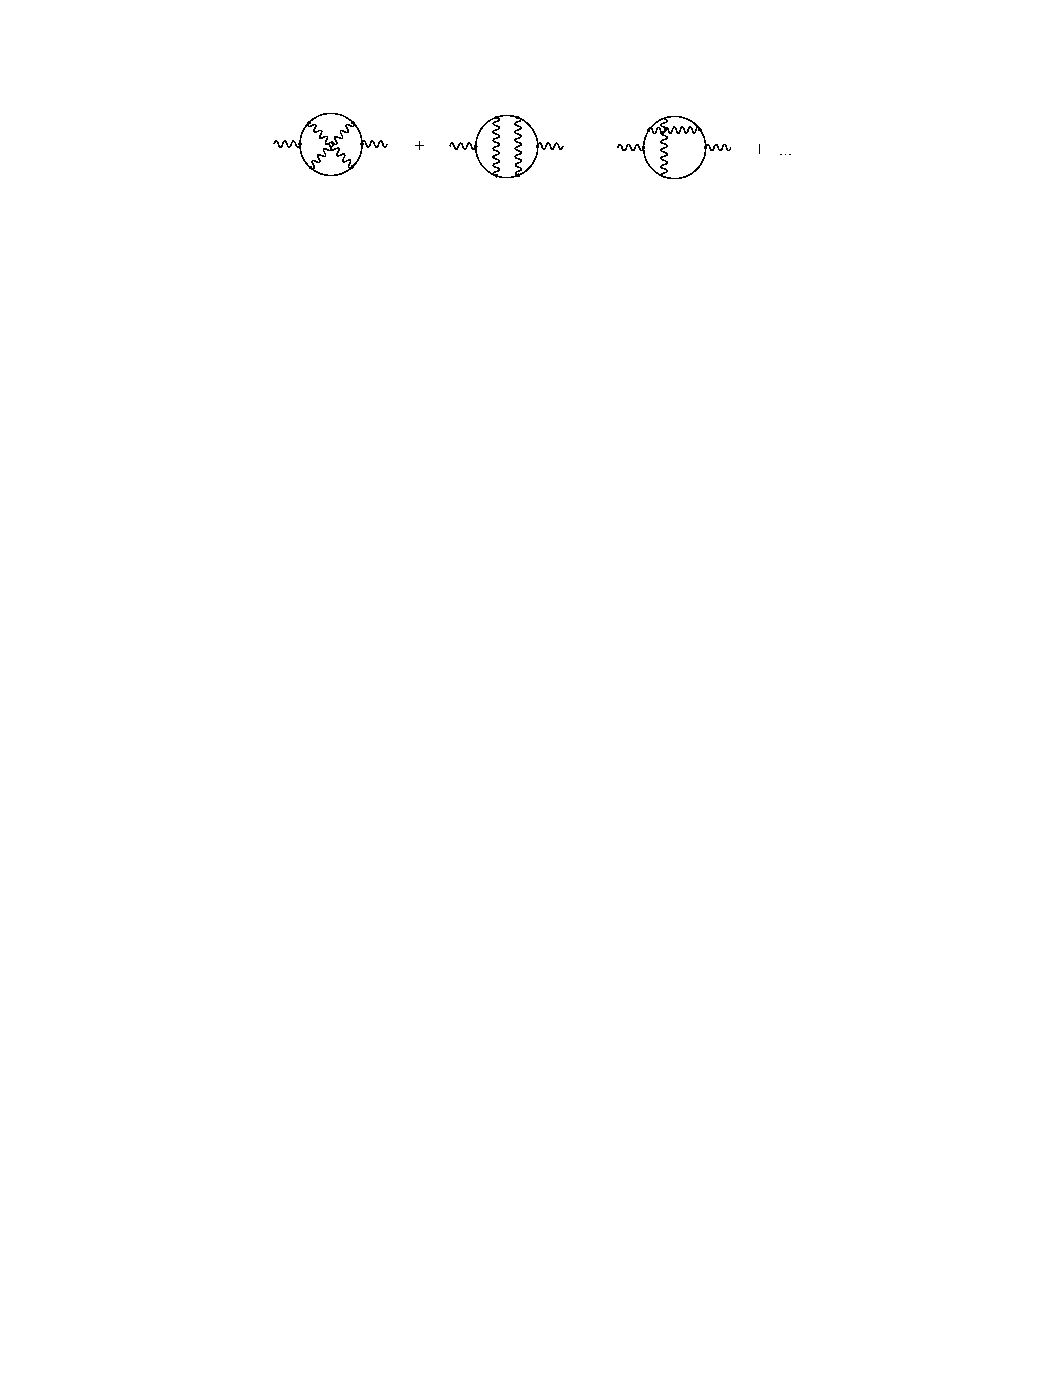
\includegraphics[width=1\textwidth]{BHSTW143loopphotonprop}
 \caption{
 Quenched diagrams contributing to the three loop QED photon propagator.
 From \refref{BHSTW14}.
 }
 \label{BHSTW143loopphotonprop}
\end{figure}
%%%%%%%%%%%%%%%%%%%%%%%%%%%%%%%%%%%%%%%%%%%%%%%%%

Thus, for the quenched scalar QED, the worldline integrals are expressed
in terms of $N$-photon propagators, the central ingredient that defines
the quenched gauge sets \refeq{quenchAnom}.
Unlike the Feynman parameter integrals for individual vertex graphs, they are
independent of the ordering of the momenta $k_1,\ldots,k_N$; the formula
\refeq{AhBaSc16(1)i} contains all $\approx N!$ ways of attaching the $N$
photons to the charged particle propagator.
The formulation combines combinatorially many Feynman diagrams into a single integral.
An example are the quenched contributions to the
three-loop photon propagator shown in \reffig{BHSTW143loopphotonprop}.

In QED the $N$-photon propagator formulation combines into one integral
all Feynman graphs related by permutations of photon legs along fermion
lines, that is, it should yield \emph{one} integral for a gauge set
$km'm$ defined in \refeq{quenchAnom}.
%, provided one may distinguish the leg-photons from the cross-photons.

\subsection{High-orders QED in worldline formalism}
\label{sect:highQEDworldline}

A non-perturbative formula for QED in a constant field, given for scalar
QED in 1982 by Affleck, Alvarez, and Manton\rf{AffAlMa82} is an example how the
worldline formalism can yield high-order information on QED amplitudes.
Huet, McKeon, and Schubert\rf{HuMcSc10} continue this in their 2010
%{\em {Euler-Heisenberg} lagrangians and asymptotic analysis in 1+1 {QED.
% Part I: Two}-loop}
%(no GaTech online access, \arXiv{1010.5315}):``
study of the l-electron loop, $N$-photon amplitudes in the limit of large
photon numbers and low photon energies, this time for 1+1 dimensional
scalar QED, in order to illustrate the large cancellations inside gauge
invariant classes of graphs.

Affleck \etal\rf{AffAlMa82} use the Feynman\rf{Feynman50} `worldline
path integral' representation of the quenched effective action for scalar
QED in the constant electric field, and calculate the amplitude in a
stationary path approximation. The stationary trajectory so obtained is a
circle with a field dependent radius, called ``instanton''  in this
context. The worldline action on this trajectory yields the correct
exponent, and the second variation determinant yields the correct  prefactor.
Using Borel analysis, they obtain non-perturbative information on the
on-shell renormalized $N$-photon amplitudes at large $N$ and low energies.

Parenthetically, independently and not by worldline formalism, but by
dint of difficult calculations and much deep physics intuition, Lebedev
and Ritus\rf{LebRit84} have arrived at a nonperturbative mass shift
interpretation for the spinor QED pair creation in constant electric
field in 1984.

For the quenched spinor QED (fermion lines decorated by photon exchanges)
closed-form expressions for general $N$ require the worldline
super-\,formalism\rf{Schubert01}, at the cost of introducing Fradkin
1966\rf{Fradkin66} Grassmann path integral,
or, alternatively,
the second order
formalism of Strassler\rf{Strassler92}.


% \item[2017-07-05 Christian] read
The  2017 G. Torgrimsson, Schneider,  Oertel and Schützhold\rf{TSOS17},
% {\em Dynamically assisted {Sauter-Schwinger} effect - non-perturbative
% versus perturbative aspects},
\arXiv{1703.09203}, sect.~3,
uses the $N$-photon formalism to determine a saddle and the asymptotic
form of two types of dynamically assisted {Sauter-Schwinger} effect.

The 2006 Dunne and Schubert\rf{DunSch06} study of scalar and spinor QED
$N$-photon amplitudes, in the quenched approximation (\ie, taking only
the diagrams with one electron loop) led to ``the following
generalization of Cvitanovi\'c's conjecture: the perturbation series
converges for all on-shell renormalized QED amplitudes at leading order
in $N_f$. It must be emphasized that the on-shell renormalization is
essential in all of the above.''
Unlike Cvitanovi\'c\rf{Cvit77b} purely numerical conjecture, theirs is a
sophisticated argument, buttressed by Borel dispersion relations.


\subsection{Electron magnetic moment in worldline formalism}
\label{sect:magMomWorldline}

Here we specialize the electron magnetic moment discussion of
\refsect{sect:magMom} to the quenched subsector.
$Z_1$,
$Z_2$, and % = (1-B)^{-1}$, and
$Z_3$,
are the respectively the vertex,
the electron wave function, and
the photon wave function
renormalization constants.
For quenched QED there are no
fermion loops, there are no vacuum polarization contribution to the charge
renormalization \refeq{IRstruct(3)}, $Z=Z_3=1$, so the bare coupling equals
the physical coupling, $\alpha_0= \alpha$.
Furthermore, $Z_1=Z_2$ by the Ward identity\rf{Ward50}.


%%%%%%%%%%%%%%% start inseert %%%%%%%%%%%%%%%%%%%%%%%%%%%%
%\section{Electron magnetic moment}
The anomalous magnetic moment of an electron $a = (g-2)/2$ is
given by the static limit of the magnetic form factor
$a=\tilde{F}_2(0)=M/(1+L)$ from \refeq{PRD10-74-III(2.2)},
with perturbative expansion
\beq
a = \frac{M(\alpha)}{1+L(\alpha)}
  =  \sum_{n=1}^\infty
          a^{(2n)}\left(\frac{\alpha}{\pi}\right)^{n}
\,,
\ee{IRstruct(1)Q}
where $Z_1=1+L =F_1(0)$, $M=F_2(0)$ are computed from the unrenormalized
on-shell values of proper vertex \refeq{BAGTB17(35-1)}, given by the sum
of all one-particle irreducible (1pI) electron-electron-photon vertex
diagrams with internal photon corrections (no electron loops).
Expanding $M$ and $L$ we have
\bea
a_{0}^{(2)} &=& M^{(2)}
            \continue
a_{0}^{(4)} &=& M^{(4)} - L^{(2)}M^{(2)}
            \label{PRD10-74-III(2.6)Q}\\
a_{0}^{(6)} &=& M^{(6)} - L^{(2)}M^{(4)} - (L^{(4)} - (L^{(2)})^2) M^{(2)}
\nnu
\eea
Each order in
\refeq{IRstruct(1)Q} is IR and UV finite, with the UV subdivergences are
cancelled by $L^{(2m)}$ counterterms in \refeq{PRD10-74-III(2.6)Q}.

A gauge set $km'm$ in expansion \refeq{quenchAnom} consists of all 1-particle irreducible vertex
diagrams without electron loops, with $k$ photons crossing the external
vertex (cross-photons) and $m [m']$ photons originating and terminating
on the incoming [outgoing] electron leg (leg-photons). One can assume
three different coupling, setting them all equal to $\alpha$ at the
end of the calculation,
\beq
a =
          \sum_{m'=0}^\infty\left(\frac{\alpha'}{\pi}\right)^{m'}
          \sum_{k=1}^\infty\left(\frac{\alpha_v}{\pi}\right)^{k}
          \sum_{m=0}^\infty\left(\frac{\alpha}{\pi}\right)^{m}
          a_{km'm}
\,.
\ee{quenchAnomQ}
The gauge set contributions are then
\bea
a^{(2)} &=& a_{100}
            \continue
a^{(4)} &=& a_{200} + a_{110} + a_{101}
            \label{gaugeSets}\\
a^{(6)} &=&  a_{300} + a_{210} + a_{201} +  a_{120} + a_{102} + a_{111}
            \continue
a^{(8)} &=& a_{400} + a_{310} + a_{301}  +  a_{220} + a_{202} + a_{211}
         +  a_{130} + a_{103} + a_{121} + a_{112}
            \continue
a^{(10)}&=& a_{500} + a_{410} + a_{401} +  a_{320} + a_{302} + a_{311}
         +  a_{230} + a_{203} + a_{221} + a_{212}
            \ceq
         +  a_{140} + a_{104} + a_{131} + a_{113} + a_{122}
\nnu
\eea




Both $L^{(2m)}$ and $M^{(2m)}$ can be evaluated in terms of
$N$-photon propagators.

\begin{enumerate}
  \item
To proceed, one needs something like a Bern-Kosower\rf{BerKos91} type
master formula for the electron line dressed with any number of photons,
with a single constant external (arbitrarily weak) magnetic field insertion.
% Schubert \etal\ have it (unpublished).
For the magnetic moment calculation, the external vertex is distinguished
by its
\(
\sigma^{\mu\nu}={1\over 2}[\gamma^{\mu},\gamma^{\nu}]
\)
form \refeq{BAGTB17(35-1)}, while all internal, virtual photon vertices
are of the usual $\gamma^{\mu}$ form.
  \item
Please write down
the worldline formula for the anomalous magnetic moment
of the electron $a=\tilde{F}_2(0)$, corresponding to Dirac trace
expression \refeq{PRD10-74-III(2.2)} for $M$.
  \item
As the external vertex transfers a (vanishing) momentum, the
incoming and outgoing electron on-mass shell legs are distinct, and thus
there are three kinds of $N$-photon propagators; $k$ photons crossing the
external vertex (cross-photons) and $m [m']$ photons originating and
terminating on the incoming [outgoing] electron leg (leg-photons). One
needs to prove in the worldline formalism that each $km'm$
integral (corresponding to a set of quenched set of 1-particle
irreducible Feynman vertex diagrams without electron loops) is separately
(i) a gauge set, and
(ii) the minimal gauge invariant set.
  \item
Hopefully the distinction motivates the  gauge set sign rule
\refeq{Cvit77b(5)}. Keep in mind, however, that this empirical rule is
already violated by the gauge set $(2,2,0)$.
  \item
Please write down
the worldline integral for one-loop anomaly $a_{0}^{(2)}$ in
\refeq{PRD10-74-III(2.6)}.
The first thing to verify is that the worldline $(1,0,0)$ integral
reproduces Schwinger's $\frac{1}{2}\left(\frac{\alpha}{\pi}\right)$
result\rf{Schwinger48}, exactly. That is an exercise in converting the
integral into Feynman-parametric form, already done several times for
other amplitudes.
  \item
Please write down the worldline integral for 2-loop anomaly
$a_{0}^{(4)}=M^{(4)}-L^{(2)}M^{(2)}$ in \refeq{PRD10-74-III(2.6)}.
Can $L^{(2)}M^{(2)}$ be absorbed into the integrand? If cancelations can
be made pointwise, that would obviate a need for constructing UV  (and
IR?) counterterms.
  \item
For 2-loop anomaly there are only 2 quenched gauge sets $km'm$:
$(2,0,0)$ and $(1,1,0)$, which equals $(1,0,1)$ by time reversal, see
\reffig{Cvit77bFig1} and \reftab{tabGaugeSets}.
So, reformulate the 2-loop calculation as two worldline integrals,
one for each gauge set.
Most likely, want to do the gauge set $(2,0,0)$ first, as it seems to
have simpler subdiagram structure (though not sure about that).
Do not attempt (for now) to evaluate these analytically (though
Broadhurst, Laporta,
Kreimer, \etc, would be interested to see whether some simplification
occurs), main thing is to understand that the UV renormalization works,
and that there are no intermediate IR divergences in this reformulation.
\end{enumerate}


\section{Volkov method}
\label{sect:Volkov}

In \refref{Volkov16} Volkov explains that $A_1^{(2n)}$ is free from
infrared divergences since they are removed by the on-shell
renormalization.
However, Volkov also states that there is no universal method in QED for
canceling IR divergences in the Feynman graphs analogous to the R
operation, and that the standard subtractive on-shell renormalization
cannot remove IR divergences point-by-point in Feynman-parametric space,
as it does for UV divergences. Moreover, it can generate additional
IR-divergences.

That QED on-mass shell amplitudes are IR-free must be an old result; even
I have several papers generalizing that to
QCD\rf{MassShell,IRstruct,QCDmshell,NPB81}. Tom Kinoshita and I solved
the problem of point-by-point removal of IR divergences in
Feynman-parametric space in my thesis\rf{CviKin74b}, with a
super-elegant formula (who needs forests?) for the UV and IR finite part
of amplitude $M_G$,
\beq
\Delta M_G =\prod_{ij}(1-I_{G/S_i})(1-K_{G/S_j}) M_G
\,,
\ee{UV-IRfiniteGcorr}
where the products are over all self-energy and vertex subdiagrams $S_i$
and $S_j$.
I have a bright memory of figuring out how to do it one quiet evening in
Ithaca, babysitting for a friend's toddler. But, as Volkov\rf{Volkov16}
and Aoyama \etal\rf{AoHaKiNiWa08} explain, our approach was apparently
not general enough to deal with the 4- and 5-loop contributions.

Volkov's algorithm is developed in {\em New method of computing the
contributions of graphs without lepton loops to the electron anomalous
magnetic moment in {QED}}\rf{Volkov17}. It is based on the ideas used for
proving UV-finiteness of renormalized Feynman
amplitudes\rf{Speer68,AnZaPo73}. He focuses on $n$-loop graphs with no
lepton loops, or, in the notation of these notes, $a^{(2n)}[V]$.
%
Volkov calculation groups Feynman graphs by self-energy graphs families
because they have similar integrand structure. In contrast to
\refrefs{CviKin74c,CarYao74,Carroll75,AoHaKiNi15} he does not evaluate
these self-energy graphs directly; all his calculations are performed
with vertex graphs, \ie, precisely what is needed to evaluate gauge sets
of \refsect{sect:finitness}. However, as illustrated in
\reffig{Cvit77bFig3}, each gauge-set vertex diagram belongs to a
different self-energy diagram, so Volkov calculation will require a major
reorganization of how integrands are generated, requiring months
of recoding.

So far Volkov  has evaluated the ladder graph
%(Figure \ref{fig_ladder})
and the fully crossed graph
%(Figure \ref{fig_crosses})
up to 5 loops. The cross graphs are of interest because they do not
contain divergent subgraphs, so their contributions only depend on the
gauge, but not on the choice of subtraction procedure.

While the contributions of individual vertex graphs (and self-energy
sets\rf{AoHaKiNi15}) are all over the place, all gauge-invariant sets are
insanely small up to order 8, and it would be very sweet to see that this
continues through order 10 (at least for the 5-loop graphs with no
electron loops).
My hunch is that starting with the gauge set $(5,0,0)$ of
\reffig{tabGaugeSets} ($5!$ vertex graphs, some of them symmetric pairs)
would be the most rewarding.
Stefano Laporta thinks it too hard, and suggests starting with the 5-loop
relative
$(1,3,1)$ (or $(1,2,2)$) of the 4-loop set $(1,2,1)$,
which would entail less than $5!$ vertex graphs (I have not counted
how many). As no high accuracy is needed, a numerical check of the QED
finiteness conjecture would good enough if the gauge sets evaluated
to two significant digits or so, but even that will need a lot of
computer time.

\section{Hopf algebraic approach}
\label{sect:HopfAlgebra}

Hopf algebraic approach of Kreimer and collaborators\rf{BrDeKr96,
Kreimer00, KreYea08, KisKre16} is very appealing - it is just that I
personally have no clue how to turn it into a direct $(g-2)$ gauge set
calculation. In the 2008 paper\rf{KreYea08}
\HREF{https://www2.mathematik.hu-berlin.de/~kreimer/} {Dirk Kreimer} and
\HREF{https://arxiv.org/find/math-ph,math/1/au:+Yeats_K/0/1/0/all/0/1}
{Karen Yeats} write:
    \begin{quote}
``One case where there is a natural interpretation is QED with a linear
number of generators, namely
\beq
X_1 = 1 + \sum_{k \geq 1}p(k)x^k
      \frac{X_1^{2k+1}}
           {(1-X_2)^{2k}(1-X_3)^{2k}}
\,,
\ee{KreYea08p413}
with $X_2$ and $X_3$ as before and with $p(k)$ linear, which corresponds
to counting with Cvitanovi\'c's gauge invariant sectors\rf{Cvit77b}.''
    \end{quote}
%{\bf 2017-05-31 Predrag}
Even in this simple case I do not see how this counts the gauge sets. My
generating function for $G_{2n}$, the number of gauge sets
(eq.~(7) in \refref{Cvit77b})  is
\beq
\sum_{n=1}^\infty G_{2n}
    =
      \frac{X}
           {(1+X)(1-X)^{3}}
\,.
\ee{Cvit77b(7)}

Broadhurst, Delbourgo and Kreimer\rf{BrDeKr96} 1996 {\em Unknotting the
polarized vacuum of quenched {QED}} unearthes much knot-theory magic,
leading to cancelations of ``transcedentals.'' While their
particular conjecture did not work out
in higher orders, the conceptual scheme might be another
route to proving the QED is finite - if there is some finite knot-theory
basis for expressing the value of every gauge set, and the gauge
invariance induced cancelations are so strong to lead to the large
cancelations of transcendentals (hyperlogarithms), then perhaps that
gives bounds on the size of each gauge set which are slower than
combinatorial. The number of different kinds of knots with $n$ crossings
is known to grow only exponentially, not faster.

Henry Ki{\ss}ler (on \refpage{sect:Hepp}) has a fresh idea for how to
approach the finiteness conjecture, using the \emph{Hepp bound},
see Panzer {\bf 2018-06-07} below.

Note that the Ki{\ss}ler and Kreimer\rf{KisKre16} definition of a ``gauge
set'' differs from \refeq{quenchAnom} used here. They organize a
gauge-dependent calculation into ``gauge sets'' of different parameter
dependence.

My notes on these papers are below, starting on \refpage{sect:BrDeKr96}.

%%%%%%%%%%%%%%%%%%%%%%%%%%%%%%%%%%%%%%%%%%%%%%%%%%%%%%%%%%%%%%%%%%%%%%%%%
% \section{Method of smooth conjugacies}
% \label{sect:scfpo}
    % reducesymm/QFT/scfpo.tex , called by finiteQED.tex
% Predrag                               jul 10 2017

\section{Method of smooth conjugacies}
\label{sect:scfpo}

\begin{quote}
\emph{If Feynman knew Poincar\'e: How to replace many diagrams by one}

In quantum field theory the standard Feynman diagram methods become
quickly unwieldy at higher orders. However,
% as students of these notes will not be shocked to hear,
it is frequently observed that the sums of Feynman diagrams, each
individually complicated, simplify miraculously to rather compact
expressions.

Here comes a possible reason why that can be traced back to Poincar\'e,
and is perhaps not something that a field theorist would instinctively
hark to as a method of computing perturbative corrections: make the
dynamics linear (``free'') by flattening out the vicinity of a path
integral extremum by a smooth nonlinear coordinate transformation.
%This does not come cheap, but
The resulting perturbative expansion is more compact than the standard
Feynman diagram perturbation theory.
\end{quote}

\noindent
The smooth conjugacy method sketched here would require some serious work
to make it a workable quantum field theory scheme. The reader might
prefer to skip straight to the worldline formalism
\refsect{sect:worldline}.

The periodic orbit theory is a classical, deterministic
theory\rf{ChaosBook} that describes nonlinear systems in ``chaotic'' (for
low-dimensional systems) or ``turbulent'' (for PDEs) regimes. The theory
allows us to calculate long time averages in a chaotic system as
expansions in terms of the periodic orbits (cycles) of the system. The
simplest example (the deterministic analogue of the quantum evolution
operator) is provided by the {\FPoper}
\beq
\Lop \rho(x')=\int\!\!dx\,\delta(f(x)-x')\rho(x)
\ee{FPoper}
for a {\em deterministic} map $f(x)$ which maps a density distribution
$\rho(x)$ forward one integer step in time. The periodic orbit theory relates the spectrum
of this operator and its weighted evolution operator generalizations to
the periodic orbits via trace formulas, \dzeta s and spec\-tral
det\-er\-min\-ants\rf{GasAlo93,ChaosBook}.

For quantum mechanics the periodic orbit theory is exact on the
semiclassical level\rf{gutbook}, whereas the quintessentially quantum
effects such as creeping, tunneling and diffraction have to be included
as corrections. In particular, the higher order $\hbar$ corrections can
be computed perturbatively by means of Feynman diagrammatic
expansions\rf{GasAlo93}.
We illustrate how this works by the parallel, but simpler example of {\em
stochastic} dynamics.
Cvitanovi\'{c}\rf{chfield} {\em {Chaotic Field Theory}: {A} sketch}
% ~predrag/articles/hongkong/hk.tex
is a programmatic statement how this theory might connect to quantum
field theory, and, by a way of motivation, an easy introduction into
different approaches to incorporating stochastic corrections into
classical dynamics.

What motivated the work\rf{noisy_Fred,conjug_Fred,diag_Fred}
summarized in \refref{chfield} is the fact that the form of perturbative
corrections for the stochastic problem  is the same as for the quantum
problem, and still the actual calculations are sufficiently simple that
one can explore more orders in perturbation theory than would be possible
for a full-fledged quantum theory.
For the simple system studied, the result is a stochastic analog of the
Gutzwiller trace formula with  the ``$\hbar$ corrections'' computed to
five orders beyond what has been attainable in the quantum-mechanical
applications. Already a discrete time,
1-dimensional discrete Langevin equation\rf{vKampen92,LM94},
\begin{equation}
x_{n+1}=f(x_n)+\sigma\xi_n
\,,\label{Langevin}
\end{equation}
with $\xi_n$ independent normalized random variables, suffices to reveal
the structure of perturbative corrections.
We treat a chaotic system with weak external noise by replacing the
deterministic evolution $\delta$-function kernel of {\FPoper}
\refeq{FPoper} by $\Lnoise{}$,  the Fokker-Planck kernel corresponding to
\refeq{Langevin}, a peaked noise distribution function
\beq
\Lnoise{}(x',x) =\delta_\sigma(f(x)-x')
\,.
\ee{Lnoise}
In the weak noise limit the kernel is sharply peaked, so it
makes sense to expand it
in terms of the Dirac delta function and
its derivatives:
\beq
	\delta_\sigma(y)
	=
	\sum_{m=0}^{\infty} {a_m \sigma^m \over m!} \, \delta^{(m)}(y)
	=
	\delta(y) +
	a_2 {\sigma^2 \over 2} \delta^{(2)}(y) +
	a_3 {\sigma^3 \over 6} \delta^{(3)}(y) + \dots
	\,.
\label{delSigExp}
\eeq
where
\[
	\delta^{(k)}(y) = {\pde^k \over \pde y^k} \delta(y)
	\,,
\]
and the coefficients $a_m$ depend on the choice of the kernel.
We have omitted the $\delta^{(1)}(y)$ term in the above because
in our applications we shall impose
the saddle-point condition, that is,
we shift $x$ by a constant to ensure that the noise peak corresponds
to $y=0$, so $\delta_\sigma^{'}(0)=0$.
For example, if $\delta_\sigma(y)$ is a Gaussian kernel,
it can be expanded as
\bea
	\delta_\sigma(y)
	&=&
	{1 \over \sqrt{2 \pi \sigma^2}} e^{-{y^2/2\sigma^2} }
	=
	\sum_{n=0}^{\infty}
	\frac{\sigma^{2n}}{n!2^n} \delta^{(2n)}(y)
	\continue
	&=&
	\delta(y) + {\sigma^2 \over 2} \delta^{(2)}(y)
	 + {\sigma^4 \over 8} \delta^{(4)}(y) + \cdots
	\,.
\label{delGaussExp}
\eea




% clipped from ~predrag/WWW/talks/UChicago99.html
% Trace formulas for stochastic evolution operators
% Feb. 10, 1999
Analogies between noise and quantum mechanics
can be explored by casting stochastic dynamics into path integral form (a
stoch\-astic Wiener integral). The periodic orbit theory is a
nonperturbative, ``WKB''  method for approximating such integrals, which
can then be improved by systematic perturbative corrections. In the weak
noise case the standard perturbation theory is an expansion in terms of
Feynman diagrams. For semiclassical quantum mechanics of a classically
chaotic system such calculation was first carried out by
Gaspard\rf{GasAlo93}. The stochastic version, implemented by Dettmann
\etal\rf{noisy_Fred}, reveals features not so readily apparent in the
quantum calculation. Perhaps some of these could be of interest to
Kreimer and collaborators, \refsect{sect:HopfAlgebra}.

The Feynman
diagram method becomes quickly unwieldy at higher orders.%
$\footnotemark\footnotetext{
The matrix method, introduced by Vattay \etal\rf{diag_Fred},
based on Rugh's\rf{hhrugh92} explicit matrix
representation of the {\evOper} will not be
discussed here. If one is interested in evaluating
numerically many orders of perturbation theory and many eigenvalues, this
method is unsurpassed.
}$
% ~predrag/articles/noise/conjug/conjug.tex clipping
%	Carl &  Predrag				27 oct 1998
However, in the Feynman diagram approach pursued in \refref{noisy_Fred},
the authors observe that the sums of Feynman diagrams simplify
miraculously to rather compact expressions.

Now the surprise; one can compute the same corrections faster and to a
higher order in perturbation theory by integrating over the neighborhood
of a given saddlepoint \emph{exactly} by means of a nonlinear change of
field variables. This elegant idea of flattening the neighborhood of a
saddlepoint, introduced by Mainieri \etal\rf{conjug_Fred}, and referred
to here as the {\em smooth conjugation method}, is perhaps an altogether
new idea in field theory. The idea, that  can be traced back to
Poincar\'e\rf{poincare}, injects into field theory a method standard in
the construction of normal forms for bifurcations\rf{Katok95}: perform a
smooth nonlinear coordinate transformation
$x = h(y)$,
$ f(x) = h(g(h^{-1}(x)))$
that flattens out the vicinity of a fixed point and makes the map {\em
linear} in an open neighborhood,
$ f(x) \to g(y) = {\bf J} \cdot y$.
\vspace{2ex}
\\
\centerline{
 ${
	\raisebox{-4.0ex}[5.5ex][4.5ex]
		 {
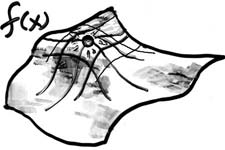
\includegraphics[height=10ex]{conjug-a}
		 }
        \atop
        \mbox{an arbitrary coordinatization}
        }$
~~~
$\Longrightarrow$
~~~
 ${
	\raisebox{-4.0ex}[5.5ex][4.5ex]
		 {
	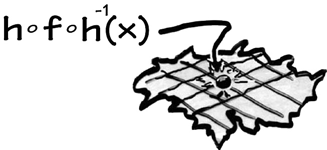
\includegraphics[height=10ex]{conjug-b}
		 }
        \atop
        \mbox{intrinsic, flat coordinates}
        }$
          }
\vspace{2ex}
\\
The resulting perturbative expansion turns out to be more compact than
the standard Feynman diagram perturbation theory; whether it is better
than the traditional loop expansions for computing field-theoretic
saddlepoint correction remains to be seen.

What is new is that the problem is being solved locally, periodic orbit
by periodic orbit, by translation to coordinates intrinsic to the
periodic orbit.

This local rectification of a map can be implemented only for isolated
non-degenerate fixed points (otherwise higher terms are required by the
normal form expansion around the point), and only in finite
neighborhoods, as the conjugating functions in general have finite radia
of convergence.

In this approach the neighborhood of each saddlepoint is rectified by an
appropriate nonlinear field transformation, with the focus shifted from
the dynamics in the original field variables to the properties of the
conjugacy transformation. The expressions thus obtained \emph{correspond
to sums} of Feynman diagrams, but are more compact.

We will try to explain this simplification in geometric terms that might
be applicable to more general field theoretic problems. The idea is this:
as the dynamics is nonlinear, why not search for a nonlinear field
transformation $\field = h(\tilde{\field})$ (a smooth conjugacy) that
makes the intrinsic coordinates as simple as possible? Schematically
--wrong in detail, but right in spirit-- find a smooth conjugacy such
that the action $S[\field] = S_0[\field] + S_I[\field]$ in the partition
function path integral becomes the free, quadratic action,
\beq
Z %[\source]
	 =  e^{W} %[\source]}
\,=\, \int [d\field] e^{S[\field]} % + \field \cdot \source}
\,=\, \int [d\tilde{\field}]
      \frac{1}{|\det \partial h(\tilde{\field})|^{1 \over 2}}
%      \, e^{\tilde{S}_0[\tilde{\field}]}
      \, e^{
      \frac{1}{2}
      \transp{\tilde{\field}}\frac{1}{\Delta}\tilde{\field}
            }
\,,
\label{Z-J}
\eeq
at the price of having the determinant of the
conjugacy Jacobian show up as a weight.

\refRef{noisy_Fred} treats the problem of computing the spectrum of this
operator by standard field-theoretic Feynman diagram expansions. Here we
formulate the perturbative expansion in terms of smooth conjugacies and
recursively evaluated derivatives. The procedure, which is relatively
easy to automatize, enables us to go one order further in the
perturbation theory, with much less computational effort than Feynman
diagrammatic expansions would require.

[TO BE CONTINUED]

%%%%%%%%%%%%%%%%%%%%%%%%%%%%%%%%%%%%%%%%%%%%%%%%%%%%%%%%%%%%%%%%%%%%%%%%%

\section{Summary}
\label{sect:Summary}

\begin{bartlett}{
\HREF{https://doi.org/10.1088/0954-3899/29/1/302}
{Everyone makes mistakes—including {Feynman}}
        }
\bauthor{
Toichiro Kinoshita\rf{Kinoshita03}
    }
\end{bartlett}
\bigskip

\noindent
Currently Sergey  A. Volkov is in the best position to check the QED
finiteness conjecture numerically, by computing the 5-loops gauge sets.

Worldline formalism could be useful on a qualitative level, as a way of
proving the finiteness of QED conjecture,
    \begin{enumerate}
  \item
Develop a saddle point expansion for the $N$-photon propagator
integrals, such that the
leading term explains the apparent $\approx \pm 1/2$ (or a multiple
thereof) size of each quenched gauge set. Affleck \etal\rf{AffAlMa82}
and G. Torgrimsson \etal\rf{TSOS17} show the way.
  \item
Use that to establish bounds on gauge sets for large orders, prove
finiteness of quenched QED. If that works, I trust electron loop
insertions will be next, and thereafter renormalons\rf{Lautrup77}, \etc,
will go \HREF{https://soundcloud.com/poets-org/notgogentle-mp3-5/s-2o7zI}
{gently into that good night}.
    \end{enumerate}
and in a precise way, as a new computational tool:
    \begin{enumerate}
  \item
Develop a worldline formulation of spinor QED in which each gauge set is
given by a computable integral, in a way to be fleshed out in
\refsect{sect:magMomWorldline}.
  \item
Parenthetically, a reformulation of the self-energy diagrams magnetic
moment calculation, \refsect{sect:selfEnergy}, would be an even greater
computational time saver - all quenched diagrams contributions calculated
at one go.
  \item
In either case, a
worldline formulation might make it possible to evaluate orders beyond
5-loops, as the number of gauge sets grows only polynomially. A win-win.
  \item
A gauge set is by definition UV and IR finite. The worldline formalism
quenched QED needs wave function
counterterms, as in \refeq{IRstruct(1)}.
  \item
Things get interesting with reformulating the quenched 3-loop calculation
as four worldline integrals / gauge sets, see \reffig{Cvit77bFig3} and
\reffig{tabGaugeSets}. In particular, the fermion line attachments of
different kinds of $N$-photon propagators now get intertwined.
  \item
One electron-loop insertion into $(1,0,0)$  might be the easiest
worldline integral to
evaluate, but I find the quenched sets a higher priority.
  \item
One photon-photon scattering electron-loop insertion into $(2,0,0)$ might
be the most tempting to evaluate, but I find the quenched sets a higher
priority.
    \end{enumerate}
My main problem at the moment (well, there are many:) is that nobody
seems to have written an explicit formula for the spinor QED anomalous
magnetic moment in the worldline formalism.
